\pdfbookmark{Общая характеристика работы}{characteristic}             % Закладка pdf
\section*{Общая характеристика работы}

\newcommand{\actuality}{\pdfbookmark[1]{Актуальность}{actuality}\underline{\textbf{\actualityTXT}}}
\newcommand{\progress}{\pdfbookmark[1]{Разработанность темы}{progress}\underline{\textbf{\progressTXT}}}
\newcommand{\aim}{\pdfbookmark[1]{Цели}{aim}\underline{{\textbf\aimTXT}}}
\newcommand{\tasks}{\pdfbookmark[1]{Задачи}{tasks}\underline{\textbf{\tasksTXT}}}
\newcommand{\aimtasks}{\pdfbookmark[1]{Цели и задачи}{aimtasks}\aimtasksTXT}
\newcommand{\novelty}{\pdfbookmark[1]{Научная новизна}{novelty}\underline{\textbf{\noveltyTXT}}}
\newcommand{\influence}{\pdfbookmark[1]{Практическая значимость}{influence}\underline{\textbf{\influenceTXT}}}
\newcommand{\methods}{\pdfbookmark[1]{Методология и методы исследования}{methods}\underline{\textbf{\methodsTXT}}}
\newcommand{\defpositions}{\pdfbookmark[1]{Положения, выносимые на защиту}{defpositions}\underline{\textbf{\defpositionsTXT}}}
\newcommand{\reliability}{\pdfbookmark[1]{Достоверность}{reliability}\underline{\textbf{\reliabilityTXT}}}
\newcommand{\probation}{\pdfbookmark[1]{Апробация}{probation}\underline{\textbf{\probationTXT}}}
\newcommand{\contribution}{\pdfbookmark[1]{Личный вклад}{contribution}\underline{\textbf{\contributionTXT}}}
\newcommand{\publications}{\pdfbookmark[1]{Публикации}{publications}\underline{\textbf{\publicationsTXT}}}


{\actuality} 
Задачи оптимизации применяются в самых разных областях человеческой деятельности от экономики до машинного обучения. Например, методы оптимизации позволяют решать системы уравнений, моделировать экономические процессы, обучать нейросети и анализировать риски в банках. Такое многообразие приложений связано с тем, что задача оптимизации - это поиск лучшего доступного решения, которое удовлетворяет требованиям исследуемой модели. Методы оптимизации предлагают обширный выбор инструментов, которые распределены по характеристикам моделей и предъявляемых к ней ограничений. Общая постановка задачи минимизации имеет вид
$$
    \min_{x\in Q} {f\left( x \right)}.
$$
Здесь и всюду далее $n$ --- это размерность пространства переменных, а $Q$ --- выпуклое замкнутое подмножество $\mathbb{R}^n$. Учет размерности задачи в современном мире стал необходимостью, поскольку модели усложняются и количество учитываемых параметров растет экспоненциально. Подобный рост размерности привел к росту популярности численных методов оптимизации градиентного типа. Речь о методах, в которых на итерациях может использоваться информация о значении целевой функции ее градиента. К недостаткам данного типа методов можно отнести необходимость прибегать к информации о функциональных свойствах для исследуемых задач, таких как гладкость, липшицевость и сильная выпуклость. Напомним определения используемых далее функционального свойства. Одним из них является условие Липшица вида
$$
    |f(y) - f(x)| \leq M \norm{y-x}_2 \;\;\; \forall x, y \in Q
$$
при некотором фиксированном $M > 0$, а норма $\norm{\cdot}_2$ --- это евклидова норма. Гладкость целевой функции определяется как условие Липшица для градиента:
$$
    \norm{\nabla f(x) - \nabla f(y)}_2 \leq L \norm{x - y}_2 \;\;\; \forall x, y \in Q
$$
при некотором фиксированном $L > 0$.
Данное условие влечет неравенство, более часто применяемое на практике,
\begin{equation}\label{l_grad}
    f(y) \leq f(x) + \langle \nabla{f(x)}, y - x \rangle  + \frac{L}{2} \|x - y \|_2^2 \quad   \forall x, y \in Q.
\end{equation}
Часто полезным будет свойство сильной выпуклости функции \cite{Pol66}:
$$
\begin{aligned}
    f(\lambda x + &(1 - \lambda)y) \le\\ 
    &\lambda f(x) + (1 - \lambda)f(y) - \frac{\mu}{2} \lambda (1 - \lambda)\|x - y\|^2_2 \;\;\; \forall x, y \in Q,
\end{aligned}
$$
где $0 \le \lambda \le 1$, для некоторого $\mu > 0$, называемого константой сильной выпуклости.
Для таких функций верно неравенство
\begin{equation}
    f(x) + \langle \nabla f(x), y - x \rangle + \frac{\mu}{2} \norm{x - y}_2^2 \leq f(y) \;\;\; \forall x, y \in Q.
\end{equation}

Одна из причин популярности градиентных методов - это низкая затратность и возможность отказаться в оценках скорости сходимости от размерности задачи, что делает их применение эффективным для многих задач. В широком смысле под эффективностью метода оптимизации понимается время, необходимое для получения достаточно хорошего решения. Однако, подобная величина зависит от огромного количества аспектов, не имеющих прямого отношения к алгоритму поиска достаточно хорошего решения. Такими аспектами могут являться мощность вычислительного устройства, доступная точность представления чисел, необходимое количество памяти и т.д. Чтобы разделить технический и теоретический аспекты, под эффективностью численного метода оптимизации на определенном классе задач часто понимают именно эффективность в смысле Бахвалова-Немировского \cite{Nemirovski1979} --- число обращений по ходу работы метода к \textit{оракулу}, достаточное для достижения приемлемой точности. 
Оракулом называется подпрограмма расчета значений целевой функции (градиента, гессиана или некоторой заменяющей их величины) с необходимой точностью. Как правило, данное обращение является наиболее <<дорогостоящей>> частью шага. В некоторых ситуациях оптимизация работы оракула является необходимостью для приемлемой работы метода, этот аспект будет более подробно обсуждаться на примере в рамках 1й главы в пункте 1.3.5.

Таким образом, аналитическая сложность оптимизационной задачи для метода на заданном классе характеризуется количеством запросов к оракулу для гарантии нахождения приближенного решения с заранее заданной точностью $\varepsilon > 0$. Что можно более формально описать 
$$
    \norm{x_N - x_*}_2 \leq \varepsilon, 
$$
где $x_N$ --- точка выхода алгоритма после $N$ итераций используемого метода, а $x_*$ --- искомое точное решение задачи. Также часто рассматривают точность с точки зрения значения функции, а именно
$$
    |f(x_N) - f(x_*)| \leq \varepsilon.
$$

Оракульный подход очень удобен для анализа сложности и сравнения численных методов. Если ответы оракула являются локальными и не накладывают никаких ограничений, не требуют каких-либо свойств от исследуемой функции, то такой подход также называют \textit{концепцией чёрного ящика}.

Cуществует несколько типов оракульных оценок:
\begin{itemize}
    \item верхняя --- количество обращений к оракулу не более данного значения (хуже не будет),
    \item нижняя --- не менее данного числа обращений (лучше не будет),
    \item оптимальная соответствует ситуации, когда нижняя и верхняя оценки совпадают с точностью до константных множителей, не зависящих от параметров задачи, таких как размерность, константа гладкости и прочее.
\end{itemize}

Ранее многие задачи относились к задачам \textit{небольшой размерности}, но в последнее время размерность задач увеличивается. Задачей \textit{небольшой размерности} обычно называют задачу, когда возможно $N \geq n$, где $N$ --- количество обращений к оракулу, а $n$ --- размерность пространства. На практике к задачам небольшой размерности можно отнести задачи, имеющие размерность в несколько сотен. Неплохую эффективность для таких задач имеют методы секущей гиперплоскости, к которым относятся метод центров тяжести и метод эллипсоидов. Однако их оптимальные оценки $N \sim \mathcal{O}\left(n \log{n}\right)$ существенно зависят от размерности пространства \cite{bubeck_2015}. 
Эта зависимость приводит к высоким требованиям по необходимой памяти и необходимости увеличения количества итераций с ростом размерности пространства для сохранения той же точности. Градиентные методы в противоположность им обладают сравнительно скромными требованиями по необходимой памяти, и соответствующие оценки не зависят от размерности задачи. Отметим также, что лучшие верхние оценки на классе гладких выпуклых функций известны для ускоренных методов \cite{Nesterov1983}.

Как уже было отмечено ранее, недостатком данного типа методов является необходимость ряда функциональных свойств у исследуемой функции. Выпишем известные оптимальные оценки сложности задач выпуклой оптимизации в зависимости от предположений о гладкости задачи.

\begin{table}[h]
    \caption{Оптимальные оценки количества обращений к субградиенту.}
    \label{est_tbl}
    \centering
    \begin{tabular}{|c|c|c|}
        \hline
         & \makecell{$|f(y) - f(x)| \leq$ \\ $\leq M \| y - x \|_2$} & \makecell{$\|\nabla f(y) - \nabla f(x)\|_2 \leq $\\ $\leq L \| y - x \|_2$} \\
        \hline
        $f(x)$ -- выпукла & $\mathcal{O} \left( \frac{M^2 R^2}{\varepsilon^2} \right)$ & $\mathcal{O} \left( \sqrt{\frac{L R^2}{\varepsilon}} \right)$ \\
        \hline
        \makecell{$f(x)$ -- $\mu$-сильно \\ выпукла в $\| \cdot \|_2$ - норме} & $\mathcal{O} \left( \frac{M^2}{\mu \varepsilon} \right)$ & $\mathcal{O} \left( \sqrt{\frac{L}{\mu}} \left[\ln{\frac{\mu R^2}{\varepsilon}}\right] \right)$ \\
        \hline
    \end{tabular}
\end{table}
В таблице \ref{est_tbl} $R$ --- это $\|x_0 - x_*\|_2 $, а $x_0$ --- стартовая точка алгоритма. Как видим, оценки в гладком случае существенно лучше, чем в негладком. В случаях, когда функционалы не обладают достаточными свойствами гладкости, что проявляется во многих задачах, актуальны вопросы разработки соответствующих эффективных методов. Для негладких задач нет возможности гарантировать высокую скорость сходимости. В данной работе рассматриваются некоторые типы негладких задач для которых исследуются возможные усовершенствования известных результатов при дополнительных условиях. Важным направлением является исследование обобщений уже известных классов задач, которые позволяют сохранить приемлемые вычислительные гарантии сходимости численных методов.

\iffalse
    Для улучшения оценок для негладких задач существует несколько подходов. Например, выделяют специальные подклассы задач, при помощи, например, условия острого минимума, предложенного в конце 1960-х годов Б.Т. Поляком \cite{Polyak1969}. Стоит подчеркнуть, что подобные условия зачастую выставляют более жесткие требования к задаче. 
\fi

Напомним, что для негладких задач в качестве обобщения понятия градиента рассматривают понятие субградиента. Вектор $g$ называют субградиентом в точке $x_0$, если
$$
    f(x) \geq f(x_0) + \langle g, x - x_0 \rangle \;\;\; \forall x \in Q.
$$

Известно, что оптимальная оценка субградиентного метода сублинейна на классах как выпуклых, так и сильно выпуклых липшицевых задач \cite{Bach_2012}. Это трудно считать достаточным для ряда приложений. В связи с этим для улучшения оценок скорости сходимости субградиентных методов используют такие допущения, как, например, условие острого минимума. Некоторые новые результаты в этом направлении изложены в данной работе.
\iffalse
    Подобные условия позволяют сделать несколько начальных эффективных шагов, что было продемонстрировано в работе \cite{sharp22} и будет затронуто во второй главе данной работы. Также в упомянутой главе было проведено сравнение оценок скорости субградиентных для классов задач с острым минимумом и сильной выпуклостью. Острый минимум может приводить к лучшей оценке скорости сходимости, однако данное свойство требует информации о точном решении, что является существенным ограничением.

    Оценки, получаемые при помощи условия острого минимума, обладают лучшими свойствами сходимости, однако в отсутствии знаний о точном решении нет возможности повысить точность выше предварительно заданной точности, известной для приближенного решения. Оценки скорости сходимости, использующие сильную выпуклость, не обладают столь впечатляющими оценками скорости сходимости, однако позволяют добиться гораздо большей точности. 
\fi

Отметим важное и развиваемое в данной работе обобщение оптимальных результатов для субградиентного метода на случай задачи с аналогом условия Липшица относительно некоторой выпуклой прокс-функции (относительная липшицевость). Такая прокс-функция, в отличие от классической постановки, не обязана удовлетворять условию сильной выпуклости относительно нормы \cite{AdaMirr_2021,Lu_2018,Zhou_NIPS_2020}. Напомним важное понятие дивергенции (расхождения) Брэгмана. Предполагается, что нам доступна некоторая выпуклая (вообще говоря, не сильно выпуклая) дифференцируемая прокс-функция $d$, порождающая некоторое расстояние, и соответствующая ей дивергенция (расхождение) Брэгмана \cite{Bauschke}
\[
    V(y, x) = d(y) - d(x) - \langle \nabla d(x), y - x \rangle.
\]

При помощи дивергенции Брэгмана вводятся такие необходимые понятия, как \textit{относительная липишицевость, относительная сильная выпуклость, относительная гладкость и условие относительного $\gamma$-роста}. Например, свойство относительной $L$-гладкости функции $f$ обобщает условие $L$-гладкости $f$ (см. \eqref{l_grad}), где квадрат евклидовой нормы в определении заменяется дивергенцией Брэгмана
$$
    f(y) \leq f(x) + \langle \nabla{f(x)}, y - x \rangle  + L V(y,x) \quad   \forall x, y \in Q,
$$
где $Q$ --- область определения $f$.

Наиболее заметными современными приложениями, обладающими свойствами относительной гладкости и относительной сильной выпуклости, являются задачи распределенной оптимизации в предположении схожести слагаемых \cite{Hendr}. 

Во второй главе данной работы исследуется оценка скорости сходимости субградиентного метода для сильно выпуклых задач с аналогичным предположением об относительной липшицевости. Точнее, рассматривается вариант субградиентного метода на классе относительно ограниченных и относительно сильно монотонных вариационных неравенств, а также класс относительно сильно выпукло-вогнутых седловых задач с соответствующими условиями относительной липшицевости функционалов. Вариационные неравенства являются важной вехой для работы, например, с лагранжевыми седловыми задачами. Известно, что задача решения вариационного неравенства имеет вид
$$
    \max_{x \in Q} \langle g(x), x_* - x \rangle \leq 0,
$$
где $x_*$ называют слабым решением вариационного неравенства, $Q$ --- выпуклое замкнутое подмножество $\mathbb{R}^n$, $g: Q \longrightarrow \mathbb{R}^n$. Предполагается, что решение $x_*$ существует. Такая постановка приводит к существенно более широкому классу задач, чем минимизационные задачи. Класс вариационных неравенств имеет достаточно широкую область применения в различных областях математики, таких как теория игр, моделирование потоков и математическая экономика. 

В третьей главе вводится понятие относительного $\gamma$-роста целевой функции, которое позволяет улучшить сублинейные оценки скорости сходимости субградиентного метода (зеркального спуска в случае неевклидовой прокс-структуры) для сильно выпуклых функций при помощи рестартов оригинального метода. Предлагается удобный с практической точки зрения алгоритм, использующий адаптивный критерий остановки на каждом из рестартов. 

% {\progress}
% Этот раздел должен быть отдельным структурным элементом по
% ГОСТ, но он, как правило, включается в описание актуальности
% темы. Нужен он отдельным структурынм элемементом или нет ---
% смотрите другие диссертации вашего совета, скорее всего не нужен.

{\aim} данной работы является развитие теории методов оптимизации для задач, не обладающих стандартными условиями гладкости, с упором на анализ субградиентных методов на классе задач с современными аналогами условий Липшица, сильной выпуклости и $\gamma$-роста ($\gamma > 1$).

{\underline{\textbf{Задачи,}}} решаемые в данной диссертации:
\begin{enumerate}
    \item Экспериментальная проверка теоретических результатов для задач распределенной оптимизации, не обладающая стандартными условиями гладкости, недавно полученных соавторами в работе \cite{GorbunovKMR20}.
    \item Экспериментальный анализ методов безградиентного, градиентного и квазинютоновского типов для работы с невыпуклым, вообще говоря, функционалом специальной структуры, а именно практический анализ возможностей эффективной оптимизации для задачи минимизации белка, имеющей различные физические основания,  OPLS force field. 
    \item Вывод оценки скорости сходимости зеркального спуска с использованием адаптивно подбираемых параметров на классе сильно выпуклых задач. Доказательство оценки скорости сходимости зеркального спуска для относительно ограниченных и относительно сильно монотонных операторов на классе вариационных неравенств.
    \item Исследование специальной методики рестартов зеркального спуска для относительно липшицевых задач минимизации с условием относительного $\gamma$-роста. 
\end{enumerate}
В данной работе мы для метода зеркального спуска рассматриваем аналоги условия Липшица, которые позволяют сохранить свойственные липшицевым задачам оптимальные оценки скорости сходимости. Также производится переход к аналогичной постановке задачи в терминах вариационных неравенств, что позволяет дополнительно расширить доступный класс задач. Получены улучшенные оценки скорости сходимости при помощи механизма рестартов зеркального спуска в случае наличия дополнительных условий острого минимума или относительного $\gamma$-роста. Сделан существенный акцент на экспериментальной составляющей.

{\novelty}
\begin{enumerate}[beginpenalty=10000] % https://tex.stackexchange.com/a/476052/104425
  \item Впервые получены оценки скорости сходимости метода зеркального спуска на классе вариационных неравенств с относительно сильно монотонными и относительно ограниченными операторами.
  \item Впервые получен адаптивный аналог оптимальной оценки скорости сходимости зеркального спуска для задач минимизации сильно выпуклых функций с использованием локальных аналогов константы Липшица.
  \item Впервые получены оценки скорости сходимости рестартованного метода зеркального спуска для относительно липшицевых задач оптимизации с относительным $\gamma$-ростом при $\gamma > 1$. 
\end{enumerate}

{\defpositions}
\begin{enumerate}[beginpenalty=10000] % https://tex.stackexchange.com/a/476052/104425
  \item Предложен вариант метода зеркального спуска для вариационных неравенств с относительно сильно монотонными и относительно ограниченными операторами. Доказана инвариантная по размерности пространства оценка скорости сходимости этого метода, оптимальная на указанном классе задач с точностью до умножения на постоянный множитель.
  \item Получена адаптивная оценка скорости сходимости зеркального спуска для задач минимизации сильно выпуклых функций с использованием локальных аналогов константы Липшица. При этом сохраняется оптимальность этой оценки на классе сильно выпуклых липшицевых задач с точностью до умножения на константу. В частности, это позволяет работать и с задачами, не удовлетворяющими условию Липшица.
  \item Введён аналог острого минимума ($\gamma$-роста) с использованием дивергенции Брэгмана. Получена оценка скорости сходимости рестартованного метода зеркального спуска для относительно липшицевых задач оптимизации с относительным $\gamma$-ростом. В ситуации сильно выпуклой прокс-функции предложены адаптивные правила остановки для рестартов исследуемого метода зеркального спуска и получен результат о его скорости сходимости.
\end{enumerate}

{\probation}
Основные результаты работы докладывались~на:
\begin{itemize}
    \item проектной смене <<Современные методы теории информации, оптимизации и управления>> в центре <<Сириус>>, 2021,
    \item QIPA (Quasilinear Equations, Inverse Problems and Their Applications), 2021,
    \item 64-й всероссийской научной конференции МФТИ, 2021,
    \item QIPA (Quasilinear Equations, Inverse Problems and Their Applications), 2018,
    \item 61-й всероссийской научной конференции МФТИ, 2018.
\end{itemize}

{\contribution} Ключевые результаты получены и доказаны автором лично. Также разработана библиотека для анализа и проверки методов оптимизации, обеспечивающая необходимую гибкость настройки. 

\ifnumequal{\value{bibliosel}}{0}
{%%% Встроенная реализация с загрузкой файла через движок bibtex8. (При желании, внутри можно использовать обычные ссылки, наподобие `\cite{vakbib1,vakbib2}`).
    {\publications} Основные результаты по теме диссертации изложены
    в~XX~публикациях,
    X из которых изданы в журналах, рекомендованных ВАК,
    X "--- в тезисах докладов.
}%
{%%% Реализация пакетом biblatex через движок biber
    \begin{refsection}[bl-author, bl-registered]
        % Это refsection=1.
        % Процитированные здесь работы:
        %  * подсчитываются, для автоматического составления фразы "Основные результаты ..."
        %  * попадают в авторскую библиографию, при usefootcite==0 и стиле `\insertbiblioauthor` или `\insertbiblioauthorgrouped`
        %  * нумеруются там в зависимости от порядка команд `\printbibliography` в этом разделе.
        %  * при использовании `\insertbiblioauthorgrouped`, порядок команд `\printbibliography` в нём должен быть тем же (см. biblio/biblatex.tex)
        %
        % Невидимый библиографический список для подсчёта количества публикаций:
        \printbibliography[heading=nobibheading, section=1, env=countauthorvak,          keyword=biblioauthorvak]%
        \printbibliography[heading=nobibheading, section=1, env=countauthorwos,          keyword=biblioauthorwos]%
        \printbibliography[heading=nobibheading, section=1, env=countauthorscopus,       keyword=biblioauthorscopus]%
        \printbibliography[heading=nobibheading, section=1, env=countauthorconf,         keyword=biblioauthorconf]%
        \printbibliography[heading=nobibheading, section=1, env=countauthorother,        keyword=biblioauthorother]%
        \printbibliography[heading=nobibheading, section=1, env=countregistered,         keyword=biblioregistered]%
        \printbibliography[heading=nobibheading, section=1, env=countauthorpatent,       keyword=biblioauthorpatent]%
        \printbibliography[heading=nobibheading, section=1, env=countauthorprogram,      keyword=biblioauthorprogram]%
        \printbibliography[heading=nobibheading, section=1, env=countauthor,             keyword=biblioauthor]%
        \printbibliography[heading=nobibheading, section=1, env=countauthorvakscopuswos, filter=vakscopuswos]%
        \printbibliography[heading=nobibheading, section=1, env=countauthorscopuswos,    filter=scopuswos]%
        %
        \nocite{*}%
        %
        {\publications} Основные результаты по теме диссертации изложены в~\arabic{citeauthor}~печатных изданиях
        % \arabic{citeauthorvak} из которых изданы в журналах, рекомендованных ВАК\sloppy% 
        \ifnum \value{citeauthorscopuswos}>0%
            , \arabic{citeauthorscopuswos} "--- в~периодических научных журналах, индексируемых Web of~Science или Scopus\sloppy%
        \fi%
        \ifnum \value{citeauthorconf}>0%
            , \arabic{citeauthorconf} "--- в~тезисах докладов.
        \else%
            .
        \fi%
        \ifnum \value{citeregistered}=1%
            \ifnum \value{citeauthorpatent}=1%
                Зарегистрирован \arabic{citeauthorpatent} патент.
            \fi%
            \ifnum \value{citeauthorprogram}=1%
                Зарегистрирована \arabic{citeauthorprogram} программа для ЭВМ.
            \fi%
        \fi%
        \ifnum \value{citeregistered}>1%
            Зарегистрированы\ %
            \ifnum \value{citeauthorpatent}>0%
            \formbytotal{citeauthorpatent}{патент}{}{а}{}\sloppy%
            \ifnum \value{citeauthorprogram}=0 . \else \ и~\fi%
            \fi%
            \ifnum \value{citeauthorprogram}>0%
            \formbytotal{citeauthorprogram}{программ}{а}{ы}{} для ЭВМ.
            \fi%
        \fi%
        % К публикациям, в которых излагаются основные научные результаты диссертации на соискание учёной
        % степени, в рецензируемых изданиях приравниваются патенты на изобретения, патенты (свидетельства) на
        % полезную модель, патенты на промышленный образец, патенты на селекционные достижения, свидетельства
        % на программу для электронных вычислительных машин, базу данных, топологию интегральных микросхем,
        % зарегистрированные в установленном порядке.(в ред. Постановления Правительства РФ от 21.04.2016 N 335)
    \end{refsection}%
    \begin{refsection}[bl-author, bl-registered]
        % Это refsection=2.
        % Процитированные здесь работы:
        %  * попадают в авторскую библиографию, при usefootcite==0 и стиле `\insertbiblioauthorimportant`.
        %  * ни на что не влияют в противном случае

        % \nocite{vakbib2}%vak
        % \nocite{patbib1}%patent
        % \nocite{progbib1}%program
        % \nocite{bib1}%other
        % \nocite{confbib1}%conf
    \end{refsection}%
        %
        % Всё, что вне этих двух refsection, это refsection=0,
        %  * для диссертации - это нормальные ссылки, попадающие в обычную библиографию
        %  * для автореферата:
        %     * при usefootcite==0, ссылка корректно сработает только для источника из `external.bib`. Для своих работ --- напечатает "[0]" (и даже Warning не вылезет).
        %     * при usefootcite==1, ссылка сработает нормально. В авторской библиографии будут только процитированные в refsection=0 работы.
}

% \ifsynopsis
% \else
%   \insertbiblioauthor      % Вывод всех работ автора
% \fi
 % Характеристика работы по структуре во введении и в автореферате не отличается (ГОСТ Р 7.0.11, пункты 5.3.1 и 9.2.1), потому её загружаем из одного и того же внешнего файла, предварительно задав форму выделения некоторым параметрам

%Диссертационная работа была выполнена при поддержке грантов \dots

%\underline{\textbf{Объем и структура работы.}} Диссертация состоит из~введения,
%четырех глав, заключения и~приложения. Полный объем диссертации
%\textbf{ХХХ}~страниц текста с~\textbf{ХХ}~рисунками и~5~таблицами. Список
%литературы содержит \textbf{ХХX}~наименование.

\pdfbookmark{Содержание работы}{description}                          % Закладка pdf
\section*{Содержание работы}
Во \underline{\textbf{введении}} обоснована актуальность диссертационной работы, сформулирована цель и аргументирована научная новизна исследований и представлены выносимые на защиту положения. Описываются распространенные постановки задачи минимизации, вводится понятие оракульной сложности, упоминаются возможные несоответствия между практическим временем работы и получаемой оценкой. Также описываются причины, благодаря которым, сейчас наиболее популярны методы градиентного типа. Декларируются крайне важные для данной работы определения, а именно 
\[
    V(y, x) = d(y) - d(x) - \langle \nabla d(x), y - x \rangle,
\]
где $d$ --- это некоторая выпуклая дифференцируемая функция, а порождаемое ей некоторое расстояние $V()$ называют дивергенцией Брэгмана. \cite{Bauschke} Данное определение позволит ослабить многие условия, необходимые для получения оптимальных оценок. Также вводится постановка задачи в терминах вариационных неравенств
$$
    \max_{x \in Q} \langle g(x), x_* - x \rangle \leq 0,
$$
где $x_*$ --- называют слабым решением вариационного неравенства, $Q$ --- выпуклое замкнутое подмножество $\mathbb{R}^n$, $g: Q \longrightarrow \mathbb{R}^n$. Предполагается, что решение $x_*$ существует. Уже из данной постановки задачи видно, что возможные варианты классов для оператора $g(x)$ существенно больше.


\underline{\textbf{Первая глава}} посвящена обзору литературы по теме выпуклой оптимизации. Описываются различные постановки задачи минимизации и ряд известных методов, широко использующихся на практике. Описываются классические градиентные методы и адаптивные квазиньютоновские. Описывается пример постановки и работы с задачей распределенной оптимизации, а также со специальной функцией, не обладающей выпуклостью, и описывающей энергию молекулы белка. В качестве иллюстрации приводится опыт работы с нестандартным невыпуклым функционалом, для которого нет гарантий в большинстве известных оценок, что позволяет применить методы нулевого порядка и провести некоторый технический анализ.

\underline{\textbf{В параграфе 1.1}} приводится обзор методов первого порядка вводится общая постановка задачи, приводятся оптимальные оценки важных классов задач. Также рассматриваются популярные постановки задач, например задача минимизации квадратичной формы. Проводятся пояснения о стандартных способах ускорения методов, таких как механизм рестартов, который в дальнейшем будет использован в 3й главе. Упоминаются ограничения и <<тонкие>> места, возникающие при работе с квазиньютоновскими методами, что имеет существенное значение в анализе задачи минимизации энергии белка. Многие из представленных в данной главе методов будут использованы для анализа функционала упомянутой задачи.

\underline{\textbf{Параграф 1.2}} Описывает постановку задачи для распределенной минимизации
  $$
    \min_{x \in \mathbb{R}^n}\left\{f(x)=\frac{1}{d} \sum_{i=1}^d f_i(x)\right\},
  $$
  где $d$ соответствует количеству исполнителей или узлов или вычислителей. 

  Во введении уже обсуждалась связь эффективности применения метода и используемого исполнительного устройства или топологии устройств. В связи с ростом популярности машинного обучения и значительного времени, которое требуется для обучения современных моделей (дни, недели), задачи параллелизации и распределения исполнения по различным устройствам для эффективного их использования выходят на первый план.

  Будем предполагать, что информация, касающаяся функции $f_i$, хранится только на узле $i$. Также зачастую каждую из $f_i$ рассматривают как
  $$
    f_i(x) = \frac{1}{m} \sum_{j=1}^m f_{ij}(x).
  $$ 
  Значимым параметром, влияющим на скорость сходимости, является дороговизна пересылки информации между узлами. Данный аспект является так называемым бутылочным горлышком для подобного типа задач. Потому методы, нацеленные на распределенную постановку, как правило, стараются заменить глобальный шаг (обновление всех компонент вектора $x$) на локальные аналоги. Это основная идея, которая лежит в основе таких методов как Local-SGD \cite{Stich2019LocalSC}. Также популярным подходом является уменьшение передаваемой информации между узлами путем выбора наиболее значимых компонент или более сложных механизмов компрессии. Подобные подходы используются в работах \cite{qlsgd, qsgd, err_fdbk}. Отметим, что многие методы предполагают полносвязную топологию доступных узлов или же star-топологию, когда есть один вычисляющий центр и зависимые дополнительные мощности. 

  В работе \cite{GorbunovKMR20}, например, предлагается следующий метод
  $$
  \begin{aligned} 
    x^{k+1} &=x^k-\frac{1}{d} \sum_{i=1}^d v_i^k, \\ 
    e_i^{k+1} &=e_i^k + \gamma g_i^k - v_i^k, \quad i=1,2, \ldots, d . 
  \end{aligned}
  $$
  Здесь $x^k$ отвечает за значение аргумента на итерации $k$, $v_i^k$ --- это результат вычисленный на узле $i$ на итерации $k$, $g_i^k$ --- это оценка $\nabla f_i(x^k)$ полученная узлом $i$, $\gamma$ --- это фиксированный размер шага и $e_i^k$ --- это накопленная к итерации $k$ на узле $i$ ошибка.  Подобная постановка задачи рассматривалась также и в \cite{err_fdbk}, где был проведен схожий анализ, но со своими особенностями, учитывающий отложенное вычисление градиента, компрессию и размеры обновляемой части градиента.
  В упомянутой работе функция компрессии $C()$ представлена так:
  $$
    v_i^k = C(e_i^k + \gamma g_i^k).
  $$
  Данная постановка, как и было показано в \cite{GorbunovKMR20} моими соавторами, обобщает и развивает ряд методов, таких как Error Compensated Stochastic Gradiend Descent (EC-SGD), EC-SGD-DIANA и EC-LSVRG. Теоретические результаты для данного ряда методов также были получены моими соавторами. Однако многие практические результаты были получены автором. В упомянутой статье рассматривается задача линейной регрессии для различных наборов данных
  $$
    \min_{x \in \mathbb{R}^n}\left\{ f(x) = \frac{1}{N} \sum_{i=1}^N \log \left(1+\exp \left(- y_i \cdot(A x)_i\right)\right) + \frac{\mu}{2}\|x\|^2 \right\},
  $$
  где $N$ --- это количество параметров модели, $x$ --- это веса модели, $A$ --- матрица параметров, а $y \in {\{-1,1\}}^N$ --- набор ожидаемых решений. Подобный тип задач имеет широкое распространение в машинном обучении. Важным аспектом являются используемые функции компрессии, а именно 
  \begin{enumerate}
    \item функция $TopK()$ --- $k$ компонентов, отсортированных по убыванию абсолютных значений в векторе ошибок $e_i$,
    \item $RandK()$ --- $k$ случайных компонентов,
    \item $l2-quant()$ --- выделение некоторого подпространства в $\mathbb{R}^n$ на основе вероятности, полученной при помощи нормализации входного вектора. 
  \end{enumerate}

  Очевидно, что подобные преобразования понижают допустимую точность для методов и также появляется шум, связанный с компрессией. Поскольку здесь присутствует достаточно много параметров, которые варьируются для многих методов и различных функций компрессии, то мы приведем один из тестов в качестве иллюстрации влияния компрессии на различные методы --- см. рис. \ref{compr}. Здесь mushrooms --- это наименование использованного набора данных, по горизонтальной оси отложено количество итераций. Видно, что различные методы реагируют на внедрение функции компрессии по-разному. Некоторое методы более устойчивы к компрессионному шуму и позволяют эффективно повышать точность с ростом количества итераций, а именно EC-L-SVRG-DIANA.
  \begin{figure}
    \begin{center}
      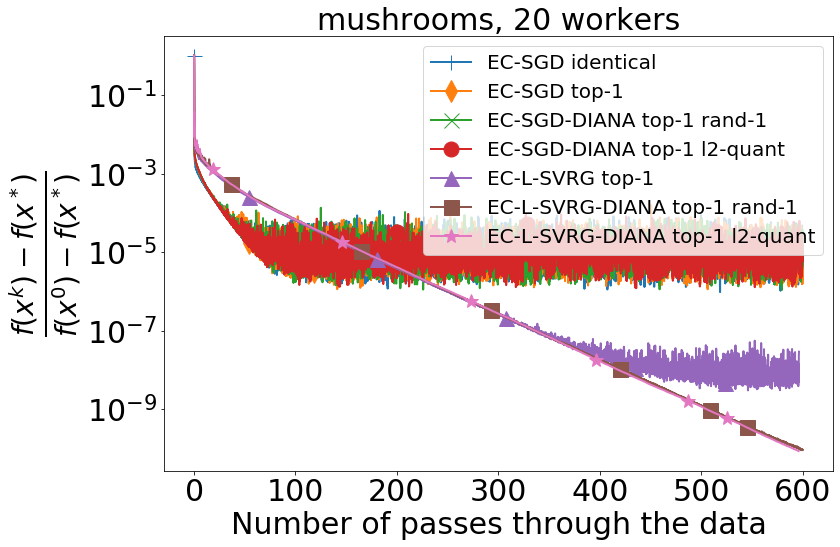
\includegraphics[width=15cm]{mushrooms_20.png}
    \end{center}
    \caption{Компрессионный шум для различных методов.}
    \label{compr}
  \end{figure}

\underline{\textbf{Параграф 1.3}} содержит анализ и предпринятые шаги по работе с практической задачей, возникшей в области вычислительной биологии. Приводится опыт работы с функционалом, не обладающим достаточной выпуклостью и основанным на ряде физических свойств объекта (что показано на рис. \ref{fig1D}). 

\begin{figure}
\begin{center}
    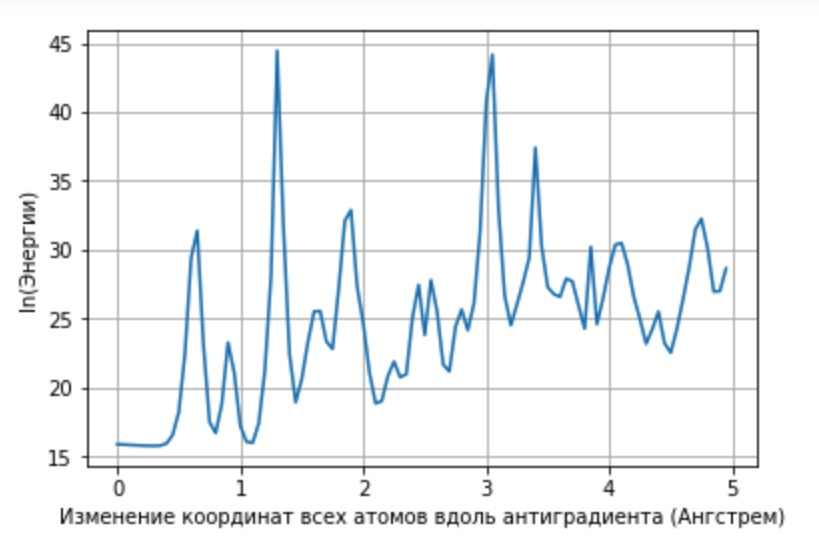
\includegraphics[height=0.24\paperheight]{1DSearch.jpg}
\end{center}
\caption{Отсутствие выпуклости задачи минимизации OPLS force field}
\label{fig1D}
\end{figure}
     
Сам пункт имеет разбиение на ряд подпунктов которые отвечают за различные этапы анализа и работы с задачей. В первом подпункте 1.3.1 описывается проблематика задачи и мотивация для ее решения. Данная задача относится к типу задач большой размерности:  $n_{ }\left(n\sim 10^4\right)$. 

Второй подпункт 1.3.2 описывает физические основания, стоящие за структурой функционала. Энергия белка основана на взаиморасположении атомов в молекуле и их различных взаимодействиях. Каждый атом в данном случае описывается тремя пространственными координатами, а самый простой белок состоит из $100$ атомов. Что позволяет оценить размерность пространства возможных конфигураций молекулы. Для подобного функционала вычисление градиента является весьма трудоемкой задачей, что объясняется сложностью и большим количеством параметров. Выпуклость пропадает в силу специфики ряда физических взаимодействий. Также стоит отметить, что в задаче необходимо найти ближайший устойчивый локальный минимум, поскольку в естественных условиях стремление к глобальному минимуму отсутствует. 

Третий пункт 1.3.3 описывает обсуждения и мотивацию, стоящую за выбором методов. Оптимизируемый функционал может рассматриваться как гладкий только локально. Константа Липшица не является равномерно ограниченной в достаточно большой, но ограниченной окрестности точки старта. Но в таком случае для минимизации такого функционала нельзя использовать градиентные методы -- нет гарантий даже локальной сходимости \cite{ghadimi2015generalized}, \cite{nesterov2017random}. 
   
Для решения таких задач глобальной оптимизации теория рекомендует использовать безградиентные методы типа simulated annealing или марковского поиска \cite{zhigljavsky2007stochastic}, \cite{zhigljavsky2012theory}.
Были проведены эксперименты с методами нулевого порядка (покоординатный спуск в различных вариациях). В основе предлагаемого подхода -- <<шевеление>> на каждой итерации только одного, случайно выбранного, атома при <<замороженных>> остальных. Заметим, что при изменении положения одного атома пересчет некоторых частей функционала будет стоить ${O}\left( 1 \right)$, поскольку затрагивает только <<соседние>> по химическим связям атомы. Здесь под <<соседними>> имеются в виду не только непосредственные соседи, но и соседи через две и даже три химические связи. Обычно число таких <<соседей>> не больше 15. 

Поскольку задача является практической основным приоритетом было качество и скорость работы. В итоге возникло интересное противопоставление - безградиентного метода со значительной параллелизацией и более линейного метода сопряженных градиентов. Однако во время работы с покоординатным спуском было обнаружено, что можно получить значительное ускорение при использовании гладкости вдоль каждой из координатных осей. Это было одним из сигналов, что градиентные методы могут быть успешно применены и для данной задачи. Эксперименты это и подтвердили, как итог финальная реализация основывалась на методах сопряженных градиентов.

\begin{table}[h]
\caption{Сравнение характеристик методов}
\label{tabular:timesandtenses}
\centering
\resizebox{\textwidth}{!}{
    \begin{tabular}{|c|c|c|}
        \hline
        \fontsize{12pt}{12pt}\selectfont {\bfseries Показатели} & {\bfseries <<Шевеление>> атома} & {\bfseries Адаптивный градиентный спуск} \\
        \hline
        \fontsize{12pt}{12pt}\selectfont Время 1 итерации, секунды    & 1.2075 & 122.9814 \\
        \hline
        \fontsize{12pt}{12pt}\selectfont Энергия 1 итерации, кДж/моль & 0.0225 & 2.7081 \\
        \hline
        \fontsize{12pt}{12pt}\selectfont $\sim\Delta$Энергии к 300 минуте, кДж/моль & $- 347$ & $- 413$ \\
        \hline
    \end{tabular}
}
\end{table}

\underline{\textbf{Во второй главе}} представлено исследование методов первого порядка для ряда классов вариационных неравенств с операторами, удовлетворяющими предлагаемому аналогу условия относительной сильной выпуклости с аналогом ограниченности (относительная ограниченность), а также с аналогом условия Липшица (относительная гладкость). Также приводится некоторое уточнение известной оптимальной оценки для субградиентного метода \cite{Bach_2012} на сильно-выпуклый случай. 

\underline{\textbf{В параграфе 2.1}} вводятся понятия относительной гладкости и определяется дивергенция Брэгмана. Также происходит переход от классической постановки к слабому решению вариационного неравенства. 

Численные методы градиентного типа достаточно часто используются для самых разнообразных постановок задач выпуклой оптимизации в пространствах больших размерностей. Это объясняется небольшими затратами памяти на итерациях, а также возможностью обоснования приемлемых оценок скорости сходимости, не содержащих (в отличие, например, от методов отсекающей гиперплоскости) параметров размерности пространства. Однако при этом существенны предположения о функциональных свойствах таких задач (гладкость, липшицевость, сильная выпуклость). Так, несколько лет назад был выделен класс относительно гладких задач оптимизации (см., например \cite{Bauschke,Drag,Lu_Nesterov_2018}). Свойство относительной $L$-гладкости ($L > 0$) обобщает ycловие $L$-гладкости ($L$-липшицевости градиента)  $f$ путём замены в известном для $L$-гладкий фyнкций $f$ неравенстве ($Q$ --- область определения $f$)
$$
    f(y) \leq f(x) + \langle \nabla{f(x)}, y - x \rangle  + \frac{L}{2} \|x - y \|_2^2 \quad   \forall x, y \in Q
$$	
выражения $\frac{1}{2} \|x - y \|_2^2 $ дивергенцией (расхождением) Брэгмана (см. \eqref{Brg_form} и \eqref{funct_rel_smooth} ниже), которая порождается некоторой выпуклой прокс-функцией (важно, что она не обязательно сильно выпукла). Отметим, что здесь и всюдy далее $\|\cdot\|_2$ --- евклидова норма в $n$-мерном пространстве $\mathbb{R}^n$.

Для выпyклых относительно гладких задач которых оценки сходимости обычных (неускоренных) методов градиентного типа оптимальны с точностью до умножения на константу, не зависящую от размерности и параметров метода (см. работы \cite{Bauschke,Drag,Dragomir,Lu_Nesterov_2018}, а также имеющиеся в них ссылки). В работе \cite{Lu_Nesterov_2018} введено понятие относительной сильной выпуклости функции, которое позволило расширить класс выпуклых оптимизационных задач, для которых можно доказать линейную скорость сходимости (сходимость со скоростью геометрической прогрессии) метода градиентного типа, причём соответствующая оценка не содержит параметров размерности задачи. В данной работе мы развиваем этот подход и исследуем некоторые алгоритмы уже для вариационных неравенств с аналогом относительной сильной выпуклости для операторов (относительной сильной монотонностью). Напомним, что понятие относительной сильной выпуклости \cite{Lu_Nesterov_2018} функции $f$ обобщает понятие обычной $\mu$-сильной выпуклости $f$ ($\mu > 0$) путём замены в неравенстве 
$$
    f(x) + \langle \nabla{f(x)}, y - x \rangle  + \frac{\mu}{2} \|x - y \|_2^2 \leq f(y) \quad   \forall x, y \in Q,
$$
выражения $\frac{1}{2} \|x - y \|_2^2 $ дивергенцией Брэгмана (см. \eqref{Brg_form} и \eqref{funct_rel_smooth} ниже), которая порождается некоторой выпуклой прокс-функцией. 

В данной главе рассматриваются методы первого порядка для двух классов вариационных неравенств с операторами, удовлетворяющими предлагаемому аналогу условия относительной сильной выпуклости (см. ниже определение  \ref{DefRelStrongMonot} относительной сильной монотонности оператора): с аналогом ограниченности (относительная ограниченность, см. определение 2 ниже), а также с аналогом условия Липшица (относительная гладкость, см. определение 3 ниже).

Хорошо известно, что на классе липшицевых и сильно выпуклых минимизационных задач оптимальная оценка скорости сходимости достигается именно для субградиентного метода \cite{Bach_2012}. В последние годы активно исследуются задачи с аналогом условия Липшица относительно некоторой выпуклой прокс-функции (относительная липшицевость), которая, в отличие от классической постановки, не обязана удовлетворять условию сильной выпуклости относительно нормы \cite{AdaMirr_2021,Lu_2018,Zhou_NIPS_2020}. Мы исследуем оценку скорости сходимости субградиентного метода для сильно выпуклых задач с аналогичным предположением об относительной липшицевости. Точнее говоря, в данной главе рассматривается вариант субградиентного метода на классе относительно ограниченных и относительно сильно монотонных вариационных неравенств, а также класс относительно сильно выпукло-вогнутых седловых задач с соответствующими условиями относительной липшицевости функционалов. 

Далее, немалую популярность в работах по оптимизации получило упомянутое выше недавно предложенное понятие относительной гладкости функций (см. работы \cite{Bauschke,Drag,Dragomir,Lu_Nesterov_2018}, а также приведённые в них ссылки), которое позволило существенно расширить класс задач выпуклой оптимизации по сравнению со стандартным предположением о липшицевости градиента с гарантией оценки скорости сходимости $O(N^{-1})$ (здесь и далее $N$ --- количество итераций), которая может считаться оптимальной для такого широкого класса задач \cite{Dragomir}. В плане приложений можно отметить подход к построению методов градиентного типа для задач распределенной оптимизации с использованием относительной гладкости и относительной сильной выпуклости \cite{Hendr}. Аналоги относительной гладкости введены в последние пару лет и для более общей постановки задачи решения вариационного неравенства (см. \cite{Inex}, а также имеющиеся там ссылки) с монотонным оператором. Оказывается, что для этого класса задач можно предложить алгоритмы экстраградиентного типа с гарантией оценки скорости сходимости $O(N^{-1})$. Мы же рассматриваем класс относительно сильно монотонных и относительно гладких операторов и приводим соответствующие оценки.

Перед переходом к постановке задачи в терминах вариационных неравенств следует упомянуть адаптивный аналог \cite{Stonyakin_2021} теоретической оценки качества выдаваемого решения для субградиентного метода \cite{Bach_2012}. Напомним, что в работе рассматриваются задачи вида
\begin{gather}\label{min_q}
    f(x)\rightarrow\min_{x\in Q},
\end{gather}
где $Q$ --- выпуклое замкнутое подмножество $\mathbb{R}^{n}$. Для субградиентного метода вида
\begin{gather}\label{orig}
    x_{k+1} := Pr_{Q}\{x_k - h_k \nabla f(x_k) \}, \;\; \textit{где} \; h_k = \frac{2}{\mu (k+1)}
\end{gather}
известна следующая оценка скорости сходимости \cite{Bach_2012}:
\begin{equation}\label{orig_estimation_f}
    f(\widehat{x}) - f(x_*) \leq \frac{2 M^2}{\mu (N+1)}  \; \text{  при   } \; \widehat{x} = \sum\limits_{k=1}^{N} \frac{2 k}{N (N+1)} x_k, 
\end{equation}
где $M$ --- константа Липщица целевой функции $f$.
Поэтому справедлива следующая
\begin{theorem}\label{ThmBachAdaptive}
    Пусть $f$ --- $\mu$-сильно выпуклая функция. Тогда после $N$ итераций алгоритма:
    $$
        x_{k+1} := Pr_{Q}\{x_k - h_k \nabla f(x_k) \}, \;\; \textit{где} \; h_k = \frac{2}{\mu (k+1)}
    $$
    будет верно неравенство:
    \begin{equation}\label{adaptive_estimation_f}
        f(\widehat{x}) - f(x_*) \leq \frac{2}{\mu N (N+1)} \sum_{k=1}^{N} \frac{k \|\nabla f(x_k)\|_2^2}{k+1},
    \end{equation}
    где
    $$
        \widehat{x} = \sum_{k=1}^{N} \frac{2 k}{N (N+1)} x_k.
    $$
    Если $f$ ещё и $M$-липшицева при $M >0$, то
    $$
         f(\widehat{x}) - f(x) \leq \varepsilon
    $$
    после $N = \mathcal{O}(\frac{M^2}{\mu\varepsilon})$ итераций алгоритма \eqref{orig}.
\end{theorem}

Отметим, что если $x_*$ --- точное решение задачи минимизации $f$, то можно получить оценку скорости сходимости по аргументу вида
\begin{equation} \label{arg_est}
    \|\widehat{x} - x_*\|_2 \leq \frac{4}{\mu N (N+1)} \sum_{k=1}^{N} \frac{k \|\nabla f(x_k)\|_2^2}{k+1} \leq \frac{4M^2}{\mu(N+1)}.
\end{equation}

Переходя к более общей постановке задачи, будем рассматривать задачу нахождения решения $x_*$ (также называемого слабым решением) вариационного неравенства: 
\begin{equation}\label{eq:1}
\max_{x \in Q} \langle g(x), x_* - x \rangle \leq 0,
\end{equation}
где $Q$ --- выпуклое замкнутое подмножество $\mathbb{R}^n$,
$g: Q \longrightarrow \mathbb{R}^n$. Предположим, что удовлетворяющее \eqref{eq:1} решение $x_*$ существует.

Всюду далее будем предполагать, что нам доступна некоторая выпуклая (вообще говоря, не сильно выпуклая) дифференцируемая прокс-функция $d$, порождающая расстояние, а также соответствующая ей дивергенция (расхождение) Брэгмана \cite{Bauschke}
\begin{equation}\label{Brg_form}
V(y, x) = d(y) - d(x) - \langle \nabla d(x), y - x \rangle.
\end{equation}

Введём следующий аналог понятия относительной сильной выпуклости функции \cite{Lu_Nesterov_2018} для вариационных неравенств.
\begin{definition}\label{DefRelStrongMonot}
Назовём оператор $g$ относительно $\mu$-сильно монотонным, где $\mu >0$, если для всяких $x, y \in Q$ верно неравенство
    \begin{equation}\label{eq:3}
         \mu V(y, x) + \mu V(x, y) \leq \langle g(y) - g(x), y - x \rangle.
     \end{equation}
\end{definition}
Как правило, далее в статье мы будем использовать следующее неравенство, естественно вытекающее из \eqref{eq:3}.
\begin{remark}
Если оператор $g$ является  относительно $\mu$-сильно монотонным, то для всяких $x, y \in Q$ верно неравенство
$$
         \mu V(x, y) \leq \langle g(y) - g(x), y - x \rangle.
$$
\end{remark}

\underline{\textbf{В параграфе 2.2}} мы рассмотрим численные методы решения вариационных неравенств с операторами, удовлетворяющими условиям относительной ограниченности, а также относительной гладкости.
\begin{definition}\label{DefRelBound}\cite{Main}
    Назовём оператор $g: Q \longrightarrow \mathbb{R}^n$ относительно $M$-огранич\-енным, где $M >0$, если для всяких $x, y \in Q$ верно неравенство
    \begin{equation}\label{rel_bound}
         \langle g(x), x - y \rangle \leq M\sqrt{2V(y,x)}.
     \end{equation}
\end{definition}
\begin{definition}\cite{Inex}
    Назовём оператор $g: Q \longrightarrow \mathbb{R}^n$ относительно $L$-гладким, где $L > 0$, если для всяких $x, y \in Q$ верно неравенство
    \begin{equation}\label{rel_smooth}
        \langle g(y)-g(z),x-z\rangle \leq LV(x,z) + LV(z,y).
    \end{equation}
\end{definition}
Отметим, что если функция $f$ $L$-относительно гладкая \cite{Bauschke}, т.е.
\begin{equation}\label{funct_rel_smooth}
    f(y) \leq f(x) + \langle \nabla f(x), y - x\rangle + LV(y, x) \quad \forall x, y \in Q,
\end{equation}
то оператор $g(x) = \nabla f(x)$ yдовлетворяет \eqref{rel_smooth}. Однако в слyчае непотенциального оператора $g$ yсловие \eqref{rel_smooth} не сводится, вообще говоря, к \eqref{funct_rel_smooth} для какой-нибyдь фyнкции $f$.


Вслед за \cite{Bach_2012} предложим метод зеркального спуска \eqref{eq:4}, но уже для рассматриваемого в настоящей работе класса  вариационных неравенств с относительно сильно монотонными и относительно ограниченными операторами (определения \ref{DefRelStrongMonot} и \ref{DefRelBound}):
\begin{equation} \label{eq:4}
    x_{k+1} := \arg \min_{x \in Q} \left\{ h_k \langle g(x_k), x \rangle + V(x, x_k)\right\},
\end{equation}
где
$$
    h_k = \frac{2}{\mu(k+1)},\quad  \forall k= 0,1, 2, \ldots.
$$

Для метода в данной постановке формулируется и проводится доказательство следующей теоремы:
\begin{theorem}\label{thm_MD_VI}
    Пусть $g$ --- $\mu$-относительно сильно монотонный и $M$-относитель\-но ограниченный оператор. Тогда после $N$ итераций алгоритма: 
    $$ 
        x_{k+1} := \arg \min_{x \in Q} \{ h_k \langle g(x_k), x\rangle + V(x, x_k)\}, \;\;\; h_k = \frac{2}{\mu (k+1)}
    $$
    будет верно неравенство:
    \begin{equation}\label{eq:2}
        \max_{x \in Q} \langle g(x), \widehat{x} - x\rangle \leq \frac{2 M^2}{\mu (N+1)},
    \end{equation}
    где 
    $$
        \widehat{x} = \sum_{k=1}^{N} \frac{2 k}{N (N+1)} x_k.
    $$
\end{theorem}

\begin{remark}
    Если $x_*$ --- сильное решение рассматриваемого вариационного не\-равенства, то можно выписать оценку скорости сходимости и <<по аргументу>>, поскольку $\langle g(x_*), x_k - x_*\rangle \geq 0$. Тогда следуя логике, использованной в доказательстве теоремы \ref{thm_MD_VI}, можно получить следующие результаты: 
        \begin{equation} \label{eq:12}
        \begin{aligned} 
            \sum_{k=1}^{N} \frac{2k\mu V(x_k, x_*)}{N(N+1)} \leq \frac{2M^2}{\mu(N+1)} \quad  \forall x \in Q,
        \end{aligned}
        \end{equation}
    Если же прокс-функция $1$-сильно выпукла относительно нормы $\|\cdot\|$, то из \eqref{eq:12} вытекает следующая оценка:
        \begin{equation} 
        \begin{aligned} 
            \|x_* - x_k\|^2 \leq \frac{4M^2}{\mu(N+1)}.
        \end{aligned}
        \end{equation}
\end{remark}
\begin{remark}
    Если прокс-функция $d$ является $1$-сильно выпуклой, то оценку \eqref{eq:2} можно уточнить:
    \begin{equation}
        \max_{x \in Q} \langle g(x), \widehat{x} - x \rangle \leq \frac{2}{\mu N (N+1)} \sum_{k=1}^{N} \frac{k \|g(x_k)\|_*^2}{k+1} \leq \varepsilon.
    \end{equation}
    Правая часть предыдущего неравенства может оказаться существенно меньшей, чем для оценки \eqref{eq:2}. Этот подход полностью аналогичен подходу, описанному при получении \eqref{arg_est}.
\end{remark}

\underline{\textbf{В параграфе 2.4}} описываются численные эксперименты, сравнивающие оригинальную оценку \eqref{orig_estimation_f} с полученной в параграфе 2.1 оценкой \eqref{adaptive_estimation_f} и приводится пример, когда оригинальная оценка неприменима. 

Для иллюстрации различия между \eqref{orig_estimation_f} и \eqref{adaptive_estimation_f} была выбрана достаточно простая задача о нахождении наименьшего покрывающего шара:
\begin{gather}\label{sphere_cover_strongly}
    f(x) := \max_{x\in Q}\left\{\|x - a_0\|_2^2, \|x - a_1\|_2^2, ..., \|x - a_m\|_2^2\right\},
\end{gather}

Основным преимуществом данной задачи является ее очевидная сильная выпуклость и тривиальность нахождения константы Липшица функции: $ M = 2 \cdot diam\{Q\} $. $Q$ в данном случае является шаром.
Рассматривалось несколько начальных конфигураций, во всех экспериментах размерность пространства $n \sim (10^3 - 10^4)$. Как правило, диаметр допустимого множества $Q$ был меньше или равен размеру искомого покрывающего шара. Такое построение позволяет работать с очень простой процедурой проектирования точек из $\mathbb{R}^n$ на $Q$.

На всех рисунках в данном параграфе зеленая линия отвечает за невязку по функции, синяя за уточненную оценку \eqref{adaptive_estimation_f}, а оранжевая за глобальную оценку \eqref{orig_estimation_f}. Хорошо показано на рис. \ref{r_20_q_6} насколько уточненная оценка ближе к реальному значению невязки, чем ее глобальная версия. 

\begin{figure}[h]
	\centering
	\includegraphics[height=0.28\paperheight]{"compare_radius_20"}
    \caption{Невязка по функции и оценки для задачи минимизации \eqref{sphere_cover_strongly} для $Q$ радиуса 6.}
    \label{r_20_q_6}
\end{figure}

\begin{figure}[h]
	\centering
	\includegraphics[height=0.25\paperheight]{"q_unlim"}
    \caption{Работа уточненной оценки \eqref{adaptive_estimation_f} для задачи минимизации \eqref{sphere_cover_strongly} для шара $Q = \mathbb{R}^n$.}
    \label{q_unlim}
\end{figure}

Также появляется интересная возможность, использовать ее в тех случаях, когда константу Липшица ($M$) целевой функции невозможно или сложно оценить. В качестве примера используется случай, когда $Q = \mathbb{R}^n$, в таком случае значение $M$ неограниченно и уходит в бесконечность. Именно этот случай показан на рис. \ref{q_unlim}. 

\begin{figure}[h]
	\centering
	\includegraphics[height=0.25\paperheight]{"q_unlim_raw"}
    \caption{Поведение невязки функции в отсутствии усреднения для задачи \eqref{sphere_cover_strongly} для шара $Q = \mathbb{R}^n$}
    \label{non_avg}
\end{figure}

Для общего понимания показано поведение неусредненной версии невязки на рис. \ref{non_avg}. Такое поведение является следствием субградиентой природы задачи. 

Именно субградиентная природа методов и необходимость изменять алгоритм проектирования привела к необходимости реализации собственной библиотеки для проведения этих и последующих экспериментов. В большинстве встроенных методов нет возможности задания специальных  множеств и при работе с задачами, имеющими субградиентную природу, такие библиотеки как scipy выдают некорректный результат. Также зачастую подобные библиотеки имеют сложное внутреннее представление для проверки необходимых свойств и вычисления необходимых глобальных констант. Такой подход позволяет им работать с большим количеством возможных постановок поддерживаемых классов задач. Как правило оптимизации подобных библиотек направлены на работу с популярными постановками, например задача минимизации квадратичной формы. В более сложных случаях собственноручно реализованный метод, даже без значительных оптимизаций под конкретную задачу, показывает меньшее время работы. 


\underline{\textbf{В третей главе}} рассматриваются результаты полученные с использованием техники рестартов. Предоставляются результаты сравнения ранее полученных оценок с оценками, полученными при помощи некоторого обобщения острого минимума. Также предложен механизм рестартов для зеркального спуска с использованием условия относительного $\gamma$-роста. 

\underline{\textbf{В параграфе 3.1}} вводятся такие понятие как острый минимум и его обобщенная вариация. Также описывается проблематика острого минимума и возможность использования этого свойства для ускорения метода при помощи механизма рестартов. Также приводятся необходимые для понимания результаты, полученные моими соавторами в работе \cite{sharp22}. 

Говорят, что $f$ удовлетворяет условию острого минимума, если
\begin{gather}\label{sm}
    f(x) - f(x_*) \geq \alpha \min_{x_* \in X_*} \|x- x_*\|_2 \quad \forall x \in Q
\end{gather}
для некоторого фиксированного $\alpha >0$ и $f(x_*) = f^* = \min\limits_{x\in Q} f(x)$ для всякого $x_* \in X_*$, где $Q$ --- выпуклое и замкнутое подмножество $\mathbb{R}^n$, $X_*$ --- компакт и $\|\cdot\|_2$ --- евклидова норма. 

\underline{\textbf{В параграфе 2.3}} показывается естественная взаимосвязь между вариационными неравенствами с монотонными операторами и выпукло-вогнутыми седловыми задачами. Выпукло-вогнутые седловые задачи играют важную роль для самых разных прикладных проблем. Поэтому в данном пункте статьи мы покажем, как полученные в предыдущих пунктах результаты о методах для вариационных неравенств можно применить к седловым задачам вида
\begin{equation}\label{eqsedlo}
    f^* = \min_{u \in Q_1} \max_{v \in Q_2} f(u, v),
\end{equation}
где $f$ --- относительно сильно выпукла по $u$ и относительно сильно вогнута по $v$.

Как известно, необходимость решения вариационных неравенств мотивируется, в частности, как раз задачами вида \eqref{eqsedlo}. В качестве примера можно рассмотреть лагранжеву седловую задачу, порожденную задачей относительно сильно выпуклого программирования.  
\begin{example} Рассмотрим задачу относительно сильно выпуклого программирования (все функционалы $\widehat{f}, g_1, g_2, ...$ относительно сильно выпуклы):
    \begin{equation}\label{problem_with_fun_constraints}
        \left\{\begin{array}{c}
        \min_{x \in Q} \widehat{f}(x), \\
        g_{1}(x), g_{2}(x), \ldots, g_{m}(x) \leq 0.
        \end{array}\right.
    \end{equation}
        
    Рассмотрим соответствующую \eqref{problem_with_fun_constraints} лагранжеву седловую задачу следующего вида
    \begin{equation}\label{lagrange_problem}
        \min_{x \in Q} \max_{ \boldsymbol{\lambda}= (\lambda_1, \ldots, \lambda_m)^T \in \mathbb{R}_+^m} L(x, \boldsymbol{\lambda}) :=  \widehat{f}(x) + \sum_{p=1}^{m} \lambda_p g_p(x) - \varepsilon \sum_{p=1}^m \lambda_{p}^2.
    \end{equation}
\end{example}
Для данного типа задач можно ввести такой аналог дивергенции Брэгмана \cite{Fedor_relative_adapuniv}:
$$
    V_{\text{new}}\left((y, \boldsymbol{\lambda}), (x, \boldsymbol{\lambda}^{'})\right) = V(y,x) + \frac{1}{2} \left\|\boldsymbol{\lambda} - \boldsymbol{\lambda}^{'}\right\|_2^2, \quad  \forall y, x \in Q, \boldsymbol{\lambda},  \boldsymbol{\lambda}^{'} \in \mathbb{R}_+^m.
$$
введенная таким образом дивергенция позволяет ослабить требования к ограничениям $\boldsymbol{\lambda}$.

В данной постановке можно воспользоваться \eqref{eq:2} и доказать следующую теорему
\begin{theorem}
    Пусть $f$ --- относительно сильно выпукла по $u$ и относительно сильно вогнута по $v$, а соответствующий оператор $g$, определенный как
    \[
        g(x) := \Bigg( 
            \begin{aligned}
                f^{'}_{u}(u,v)\\
                -f^{'}_{v}(u,v)
            \end{aligned}
        \Bigg), \text{ где } x := (u, v),
    \]
    является M-ограниченным. Тогда для задачи \eqref{eqsedlo}, решаемой методом \eqref{eq:4}, после $N$ итераций будет справедливо следующее неравенство:
    \begin{equation}
        \max_{v} f(\widehat{u}, v) - \min_{u} f(u, \widehat{v}) \leq \frac{2M^2}{\mu (N+1)},
    \end{equation}
    где
    \[
        (\widehat{u}, \widehat{v}) := \frac{1}{N(N+1)} \sum_{k=1}^{N} 2k (u_k,v_k).
    \]
\end{theorem}

\underline{\textbf{В параграфе 2.4}} проводится исследование, сравнивающее специфику работы методов зеркального спуска в двух различных вариациях: 
\begin{enumerate}
    \item с использованием сильной выпуклости
    \item с использованием обобщенного условия острого минимума
\end{enumerate}

Здесь необходимо упомянуть об оценке, доказанной в \cite{sharp22} моими соавторами: С.С. Аблаев, Ф.С. Стонякин, М.С. Алкуса, И.В. Баран. Отмечу, что эта оценка показывает линейную скорость сходимости, причем наиболее значимый вклад в полученную оценку (достаточно громоздкую, чтобы приводить ее полностью) дает последнее слагаемое $\frac{\Delta^2}{2\|\nabla f(x_k)\|^2_2}$. 

Теперь перейдём к экспериментальному сравнению предложенных подходов для задач с $\Delta$-острым минимумом с работой известного субградиентного метода \cite{Bach_2012} для некоторых сильно выпуклых задач. Выбор класса сильно выпуклых задач и метода \cite{Bach_2012} для сравнения обусловлен известными и  применимыми на практике теоретическими оценками качества приближённого решения по аргументу. Напомним адаптивную оценку для сильно выпуклых функций, полученную ранее в теореме \ref{ThmBachAdaptive}:
\begin{equation}
    f(\widehat{x}) - f(x_*) \leq \frac{2}{\mu N (N+1)} \sum_{k=1}^{N} \frac{k \|\nabla f(x_k)\|_2^2}{k+1},
\end{equation} 

Основным преимуществом данной задачи является ее очевидная сильная выпуклость и тривиальность нахождения константы Липшица функции: $ M = 2 \cdot diam\{Q\} $. $Q$ в данном случае является шаром.
Рассматривалось несколько начальных конфигураций, во всех экспериментах размерность пространства $n \sim (10^3 - 10^4)$. Как правило, диаметр допустимого множества $Q$ был меньше или равен размеру искомого покрывающего шара. Такое построение позволяет работать с очень простой процедурой проектирования точек из $\mathbb{R}^n$ на $Q$.

Для сравнения скорости сходимости метода \cite{Bach_2012} и предложенного в \cite{sharp22} метода, учитывающего $\Delta$-острый минимум, проведены численные эксперименты для задачи о наименьшем покрытии точек шаром для $2$-сильно выпуклой функции:
\begin{gather}\label{sphere_cover_strongly}
    f(x) := \max_{x\in Q}\left\{\|x - a_0\|_2^2, \|x - a_1\|_2^2, ..., \|x - a_m\|_2^2\right\},
\end{gather}
а также для не сильно выпуклой (но выпуклой) функции
\begin{gather}\label{sphere_cover}
    f(x) := \max_{x\in Q}\left\{\|x - a_0\|_2, \|x - a_1\|_2, ..., \|x - a_m\|_2\right\}.
\end{gather}

Начнём с иллюстрации преимуществ адаптивной оценки метода \cite{Bach_2012} из теоремы \ref{ThmBachAdaptive}. Будем рассматривать множество Q, которое равно евклидову шару с центром в 0. Начальная точка выбиралась случайно, но внутри Q. На рис. \ref{res_ex_strong_r5} ниже показано поведение и характер убывания для оригинальной оценки (\ref{orig_estimation_f}) --- сплошная линия, адаптивной оценки (\ref{adaptive_estimation_f}) --- штрих-пунктирная линия и непосредственно невязки по функции и по аргументу соответственно --- штриховая линия. На рис. \ref{res_ex_strong_r5} показано поведение глобальной оценки, адаптивной и невязки по функции и аргументу в случае ограниченного $Q (R = 5)$. Данный график наглядно демонстрирует, насколько более точной может оказаться адаптивная оценка (\ref{adaptive_estimation_f}) для задачи \eqref{sphere_cover_strongly} и позволяет оценить скорость сходимости в логарифмических шкалах.

\begin{figure}[h]
    \minipage{0.49\textwidth}
    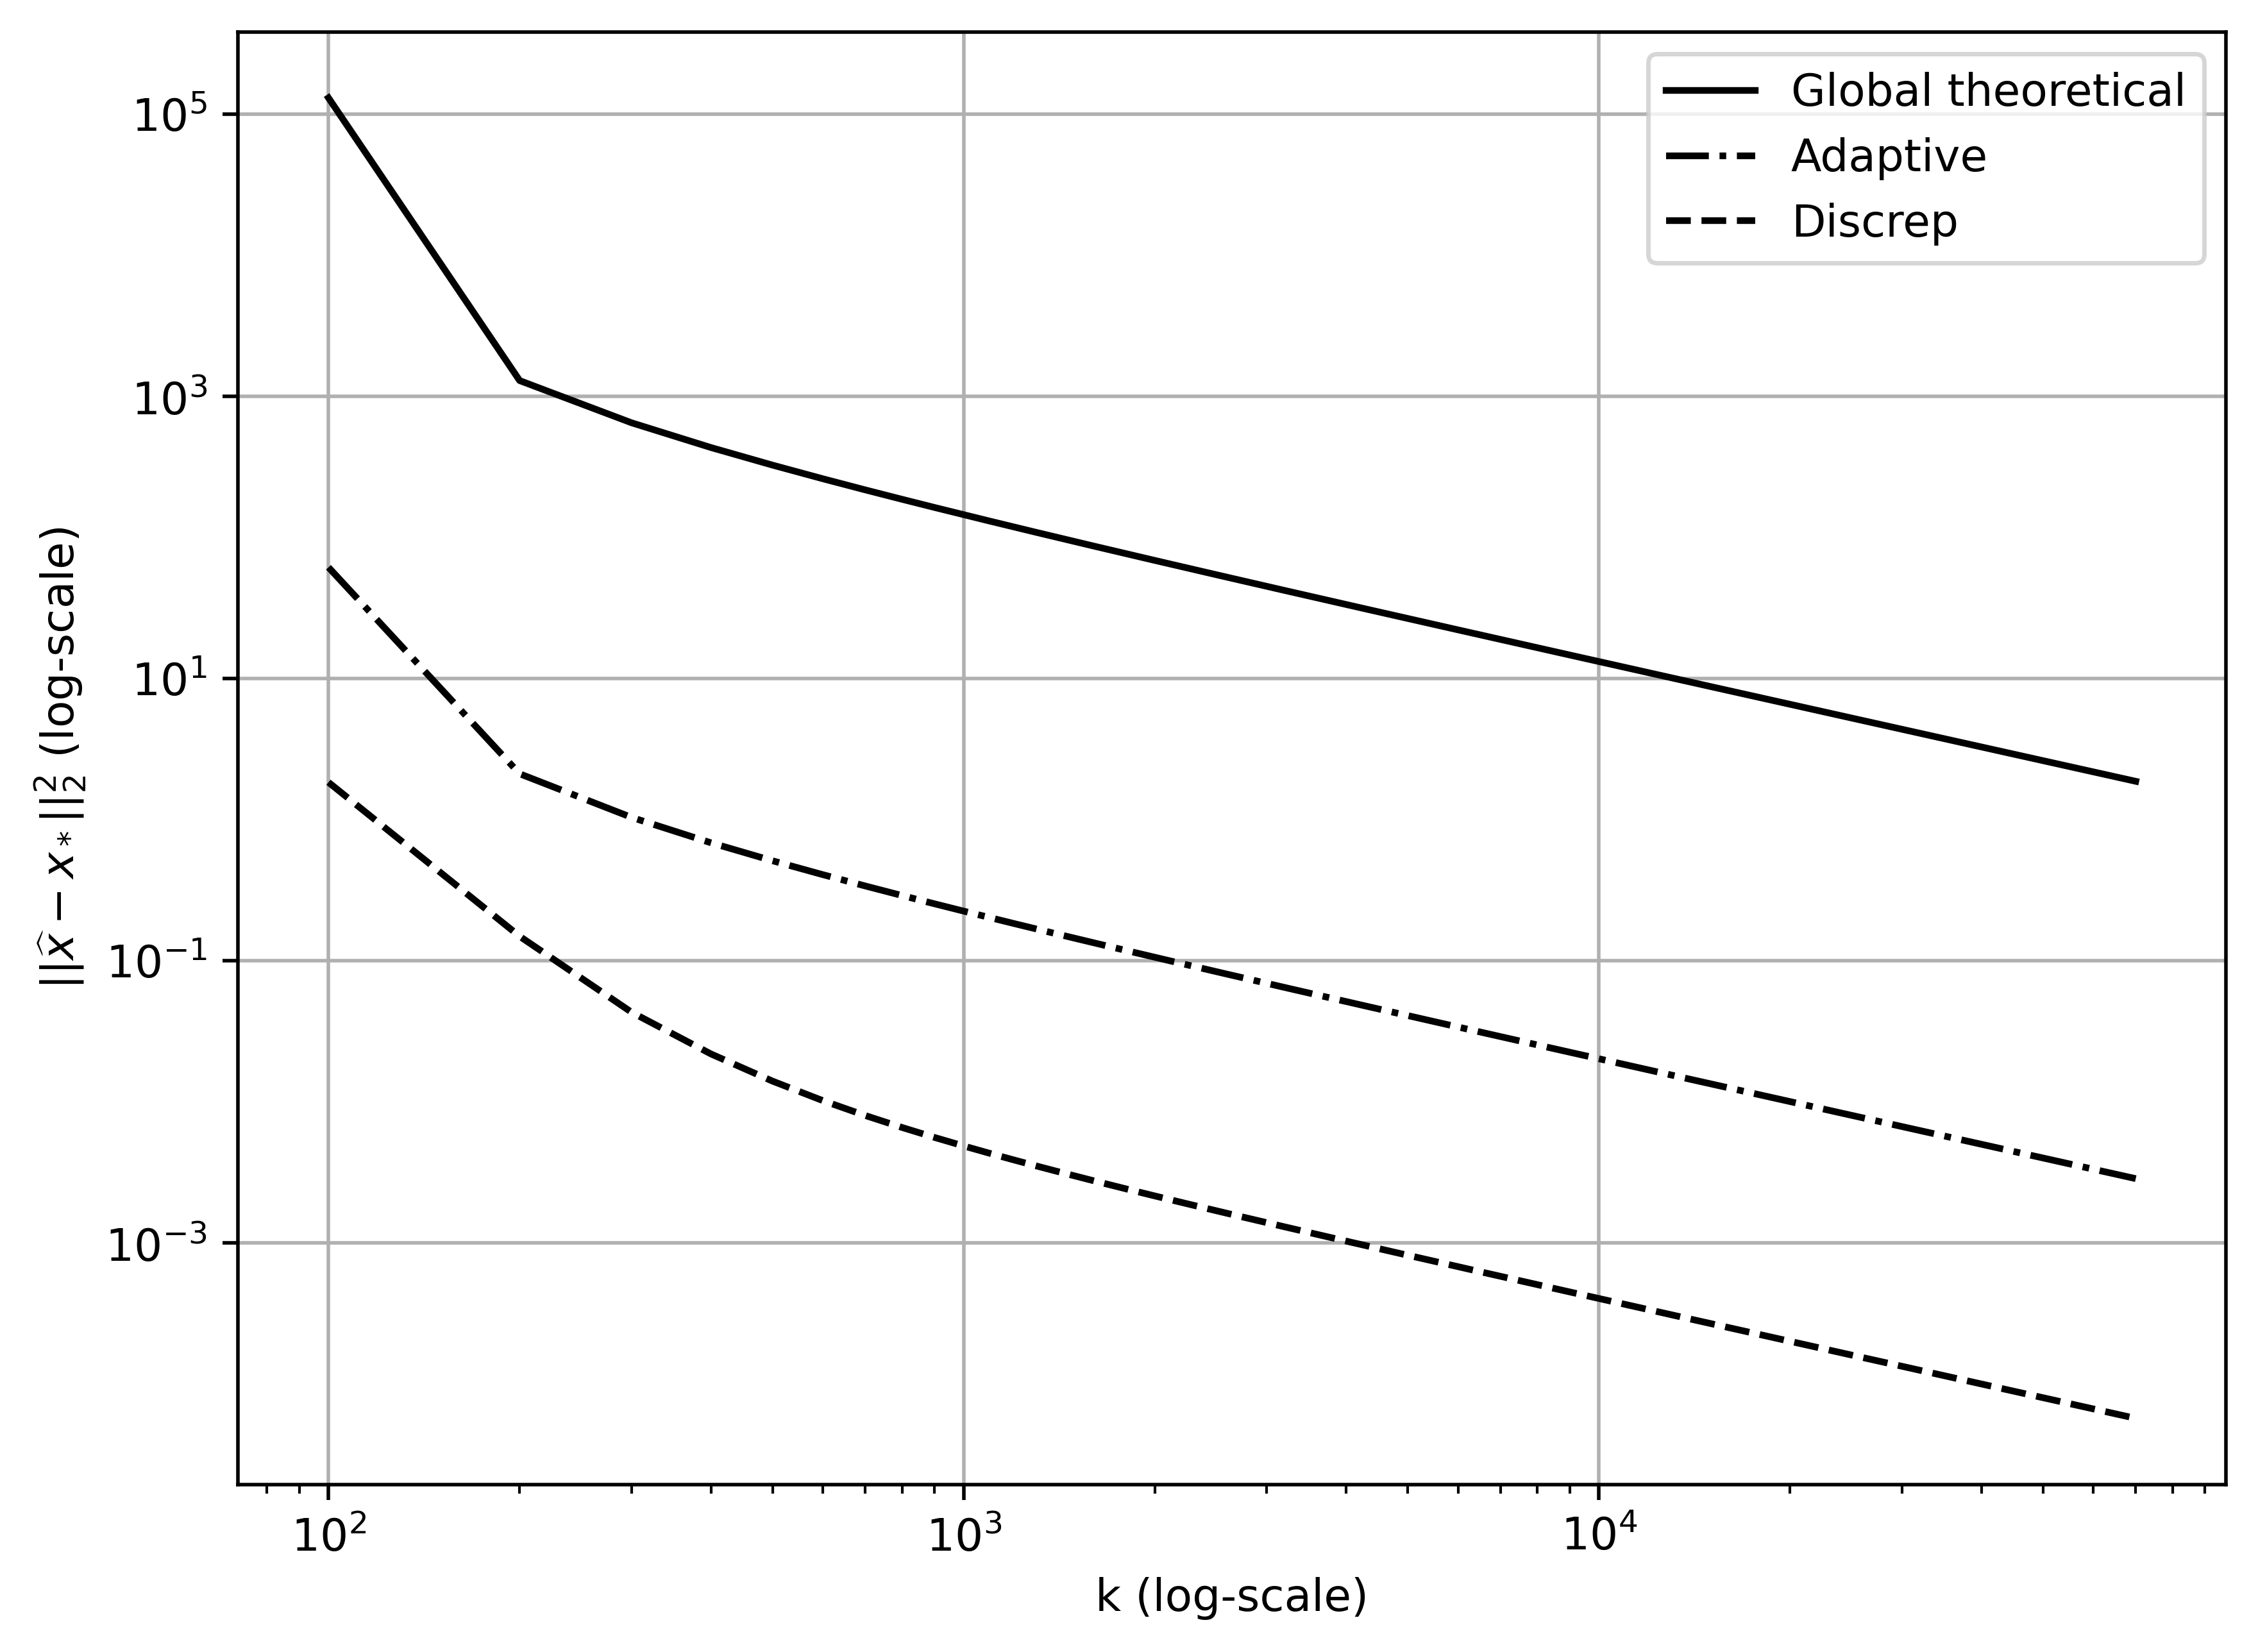
\includegraphics[width=\linewidth]{x_discr_rad_5_q_4_it_70_000_dim_1000.png}
    \endminipage\hfill
    \minipage{0.49\textwidth}
    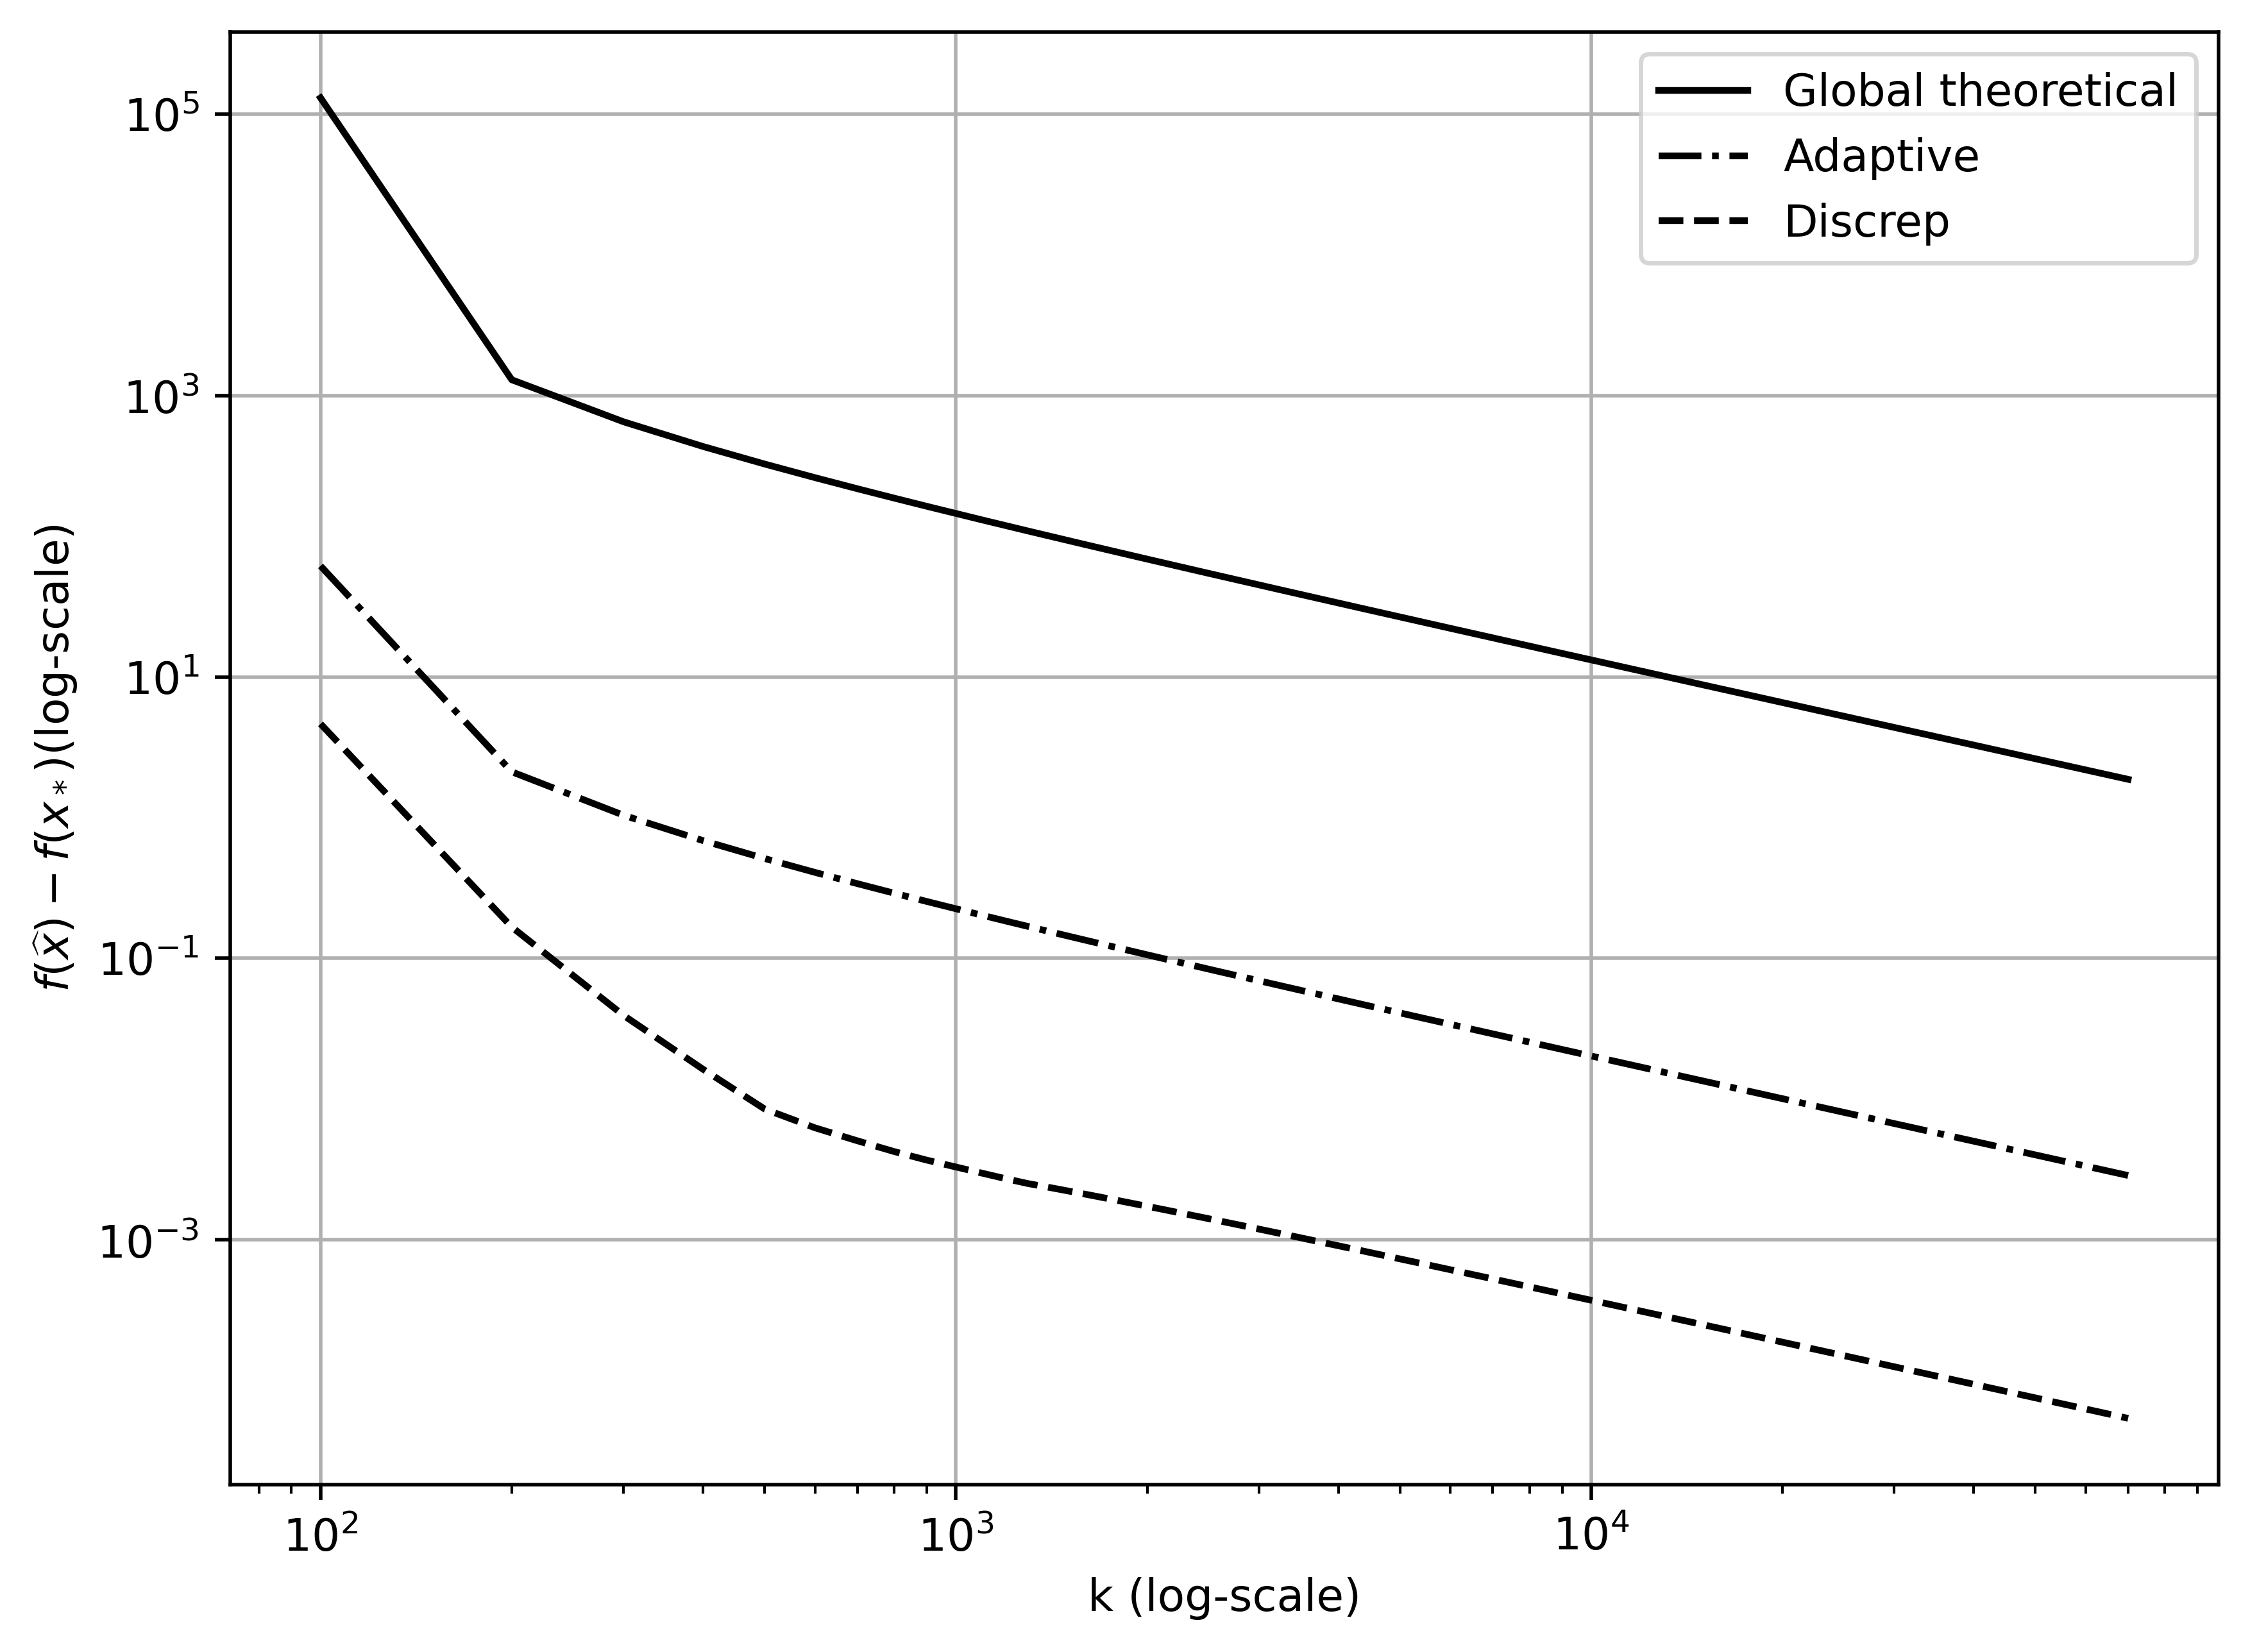
\includegraphics[width=\linewidth]{f_discr_rad_5_q_4_it_70_000_dim_1000.png}
    \endminipage\hfill
    \caption{Результаты решения задачи минимизации \eqref{sphere_cover_strongly}, где  $n= 1\,000, r = 5$ и  шар $Q$ радиуса 4.}
    \label{res_ex_strong_r5}
\end{figure}

Теперь перейдём к выпуклой постановке \eqref{sphere_cover} с целью исследования эффективности предложенного метода, учитывающего $\Delta$-острый минимум. Рассматривается целевая функция вида
\begin{gather}\label{allpha_sphere_cover}
    f(x) := \alpha \max_{x\in Q}\{\|x - a_0\|_2, \|x - a_1\|_2, ..., \|x - a_m\|_2\}.
\end{gather}

Для сравнения, ниже на рис. \ref{res_sharp_convex} и \ref{res_strong_convex} приведены результаты работы для того же набора входных точек, которые необходимо покрыть в обоих постановках --- (\ref{allpha_sphere_cover}) и (\ref{sphere_cover_strongly}). Начальная точка также одна и та же. Метод, опирающийся на $\Delta$-острый минимум, обеспечивает сходимость буквально за 10 итераций к <<приближённому>> решению с заданной точностью и даже позволяет эту точность повысить. Метод, опирающийся на сильную выпуклость, достигает схожих (с геометрической точки зрения) результатов за значительно большее количество итераций, однако он позволяет повышать точность приближённого решения на дальнейших итерациях.

\begin{figure}[h]
    \minipage{0.49\textwidth}
    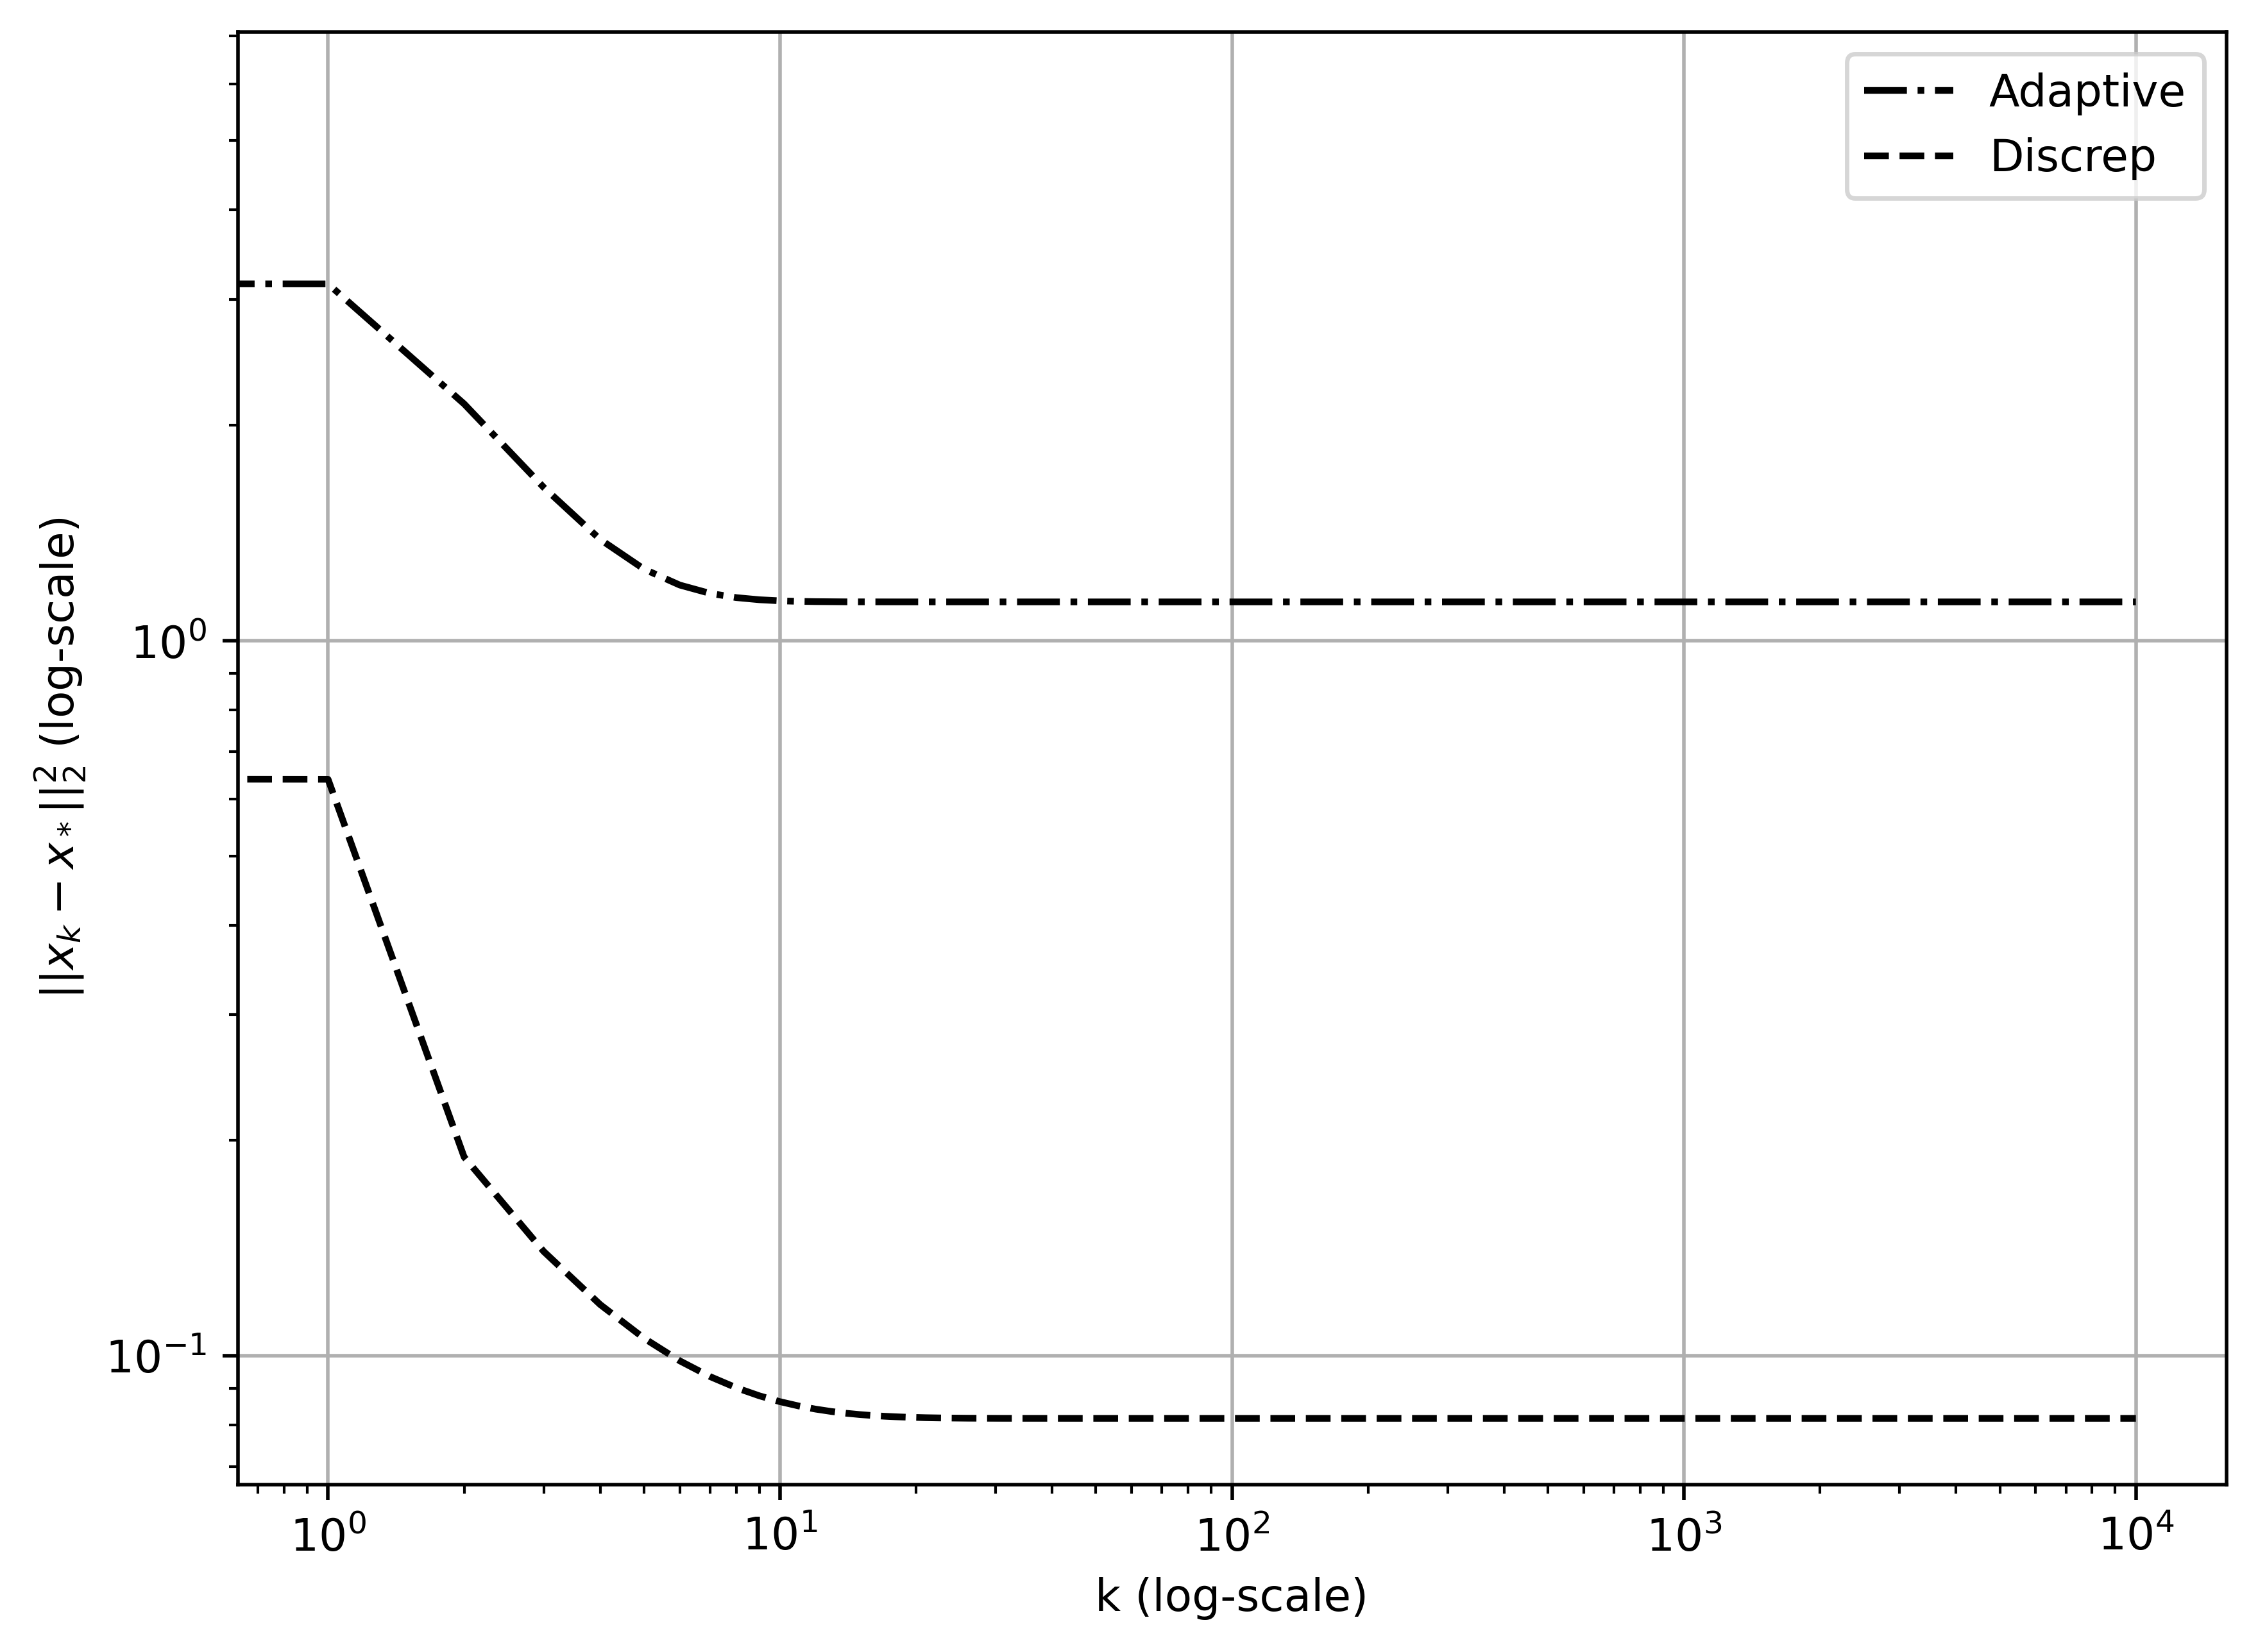
\includegraphics[width=\linewidth]{sharp_convex_x.png}
    \endminipage\hfill
    \minipage{0.49\textwidth}
    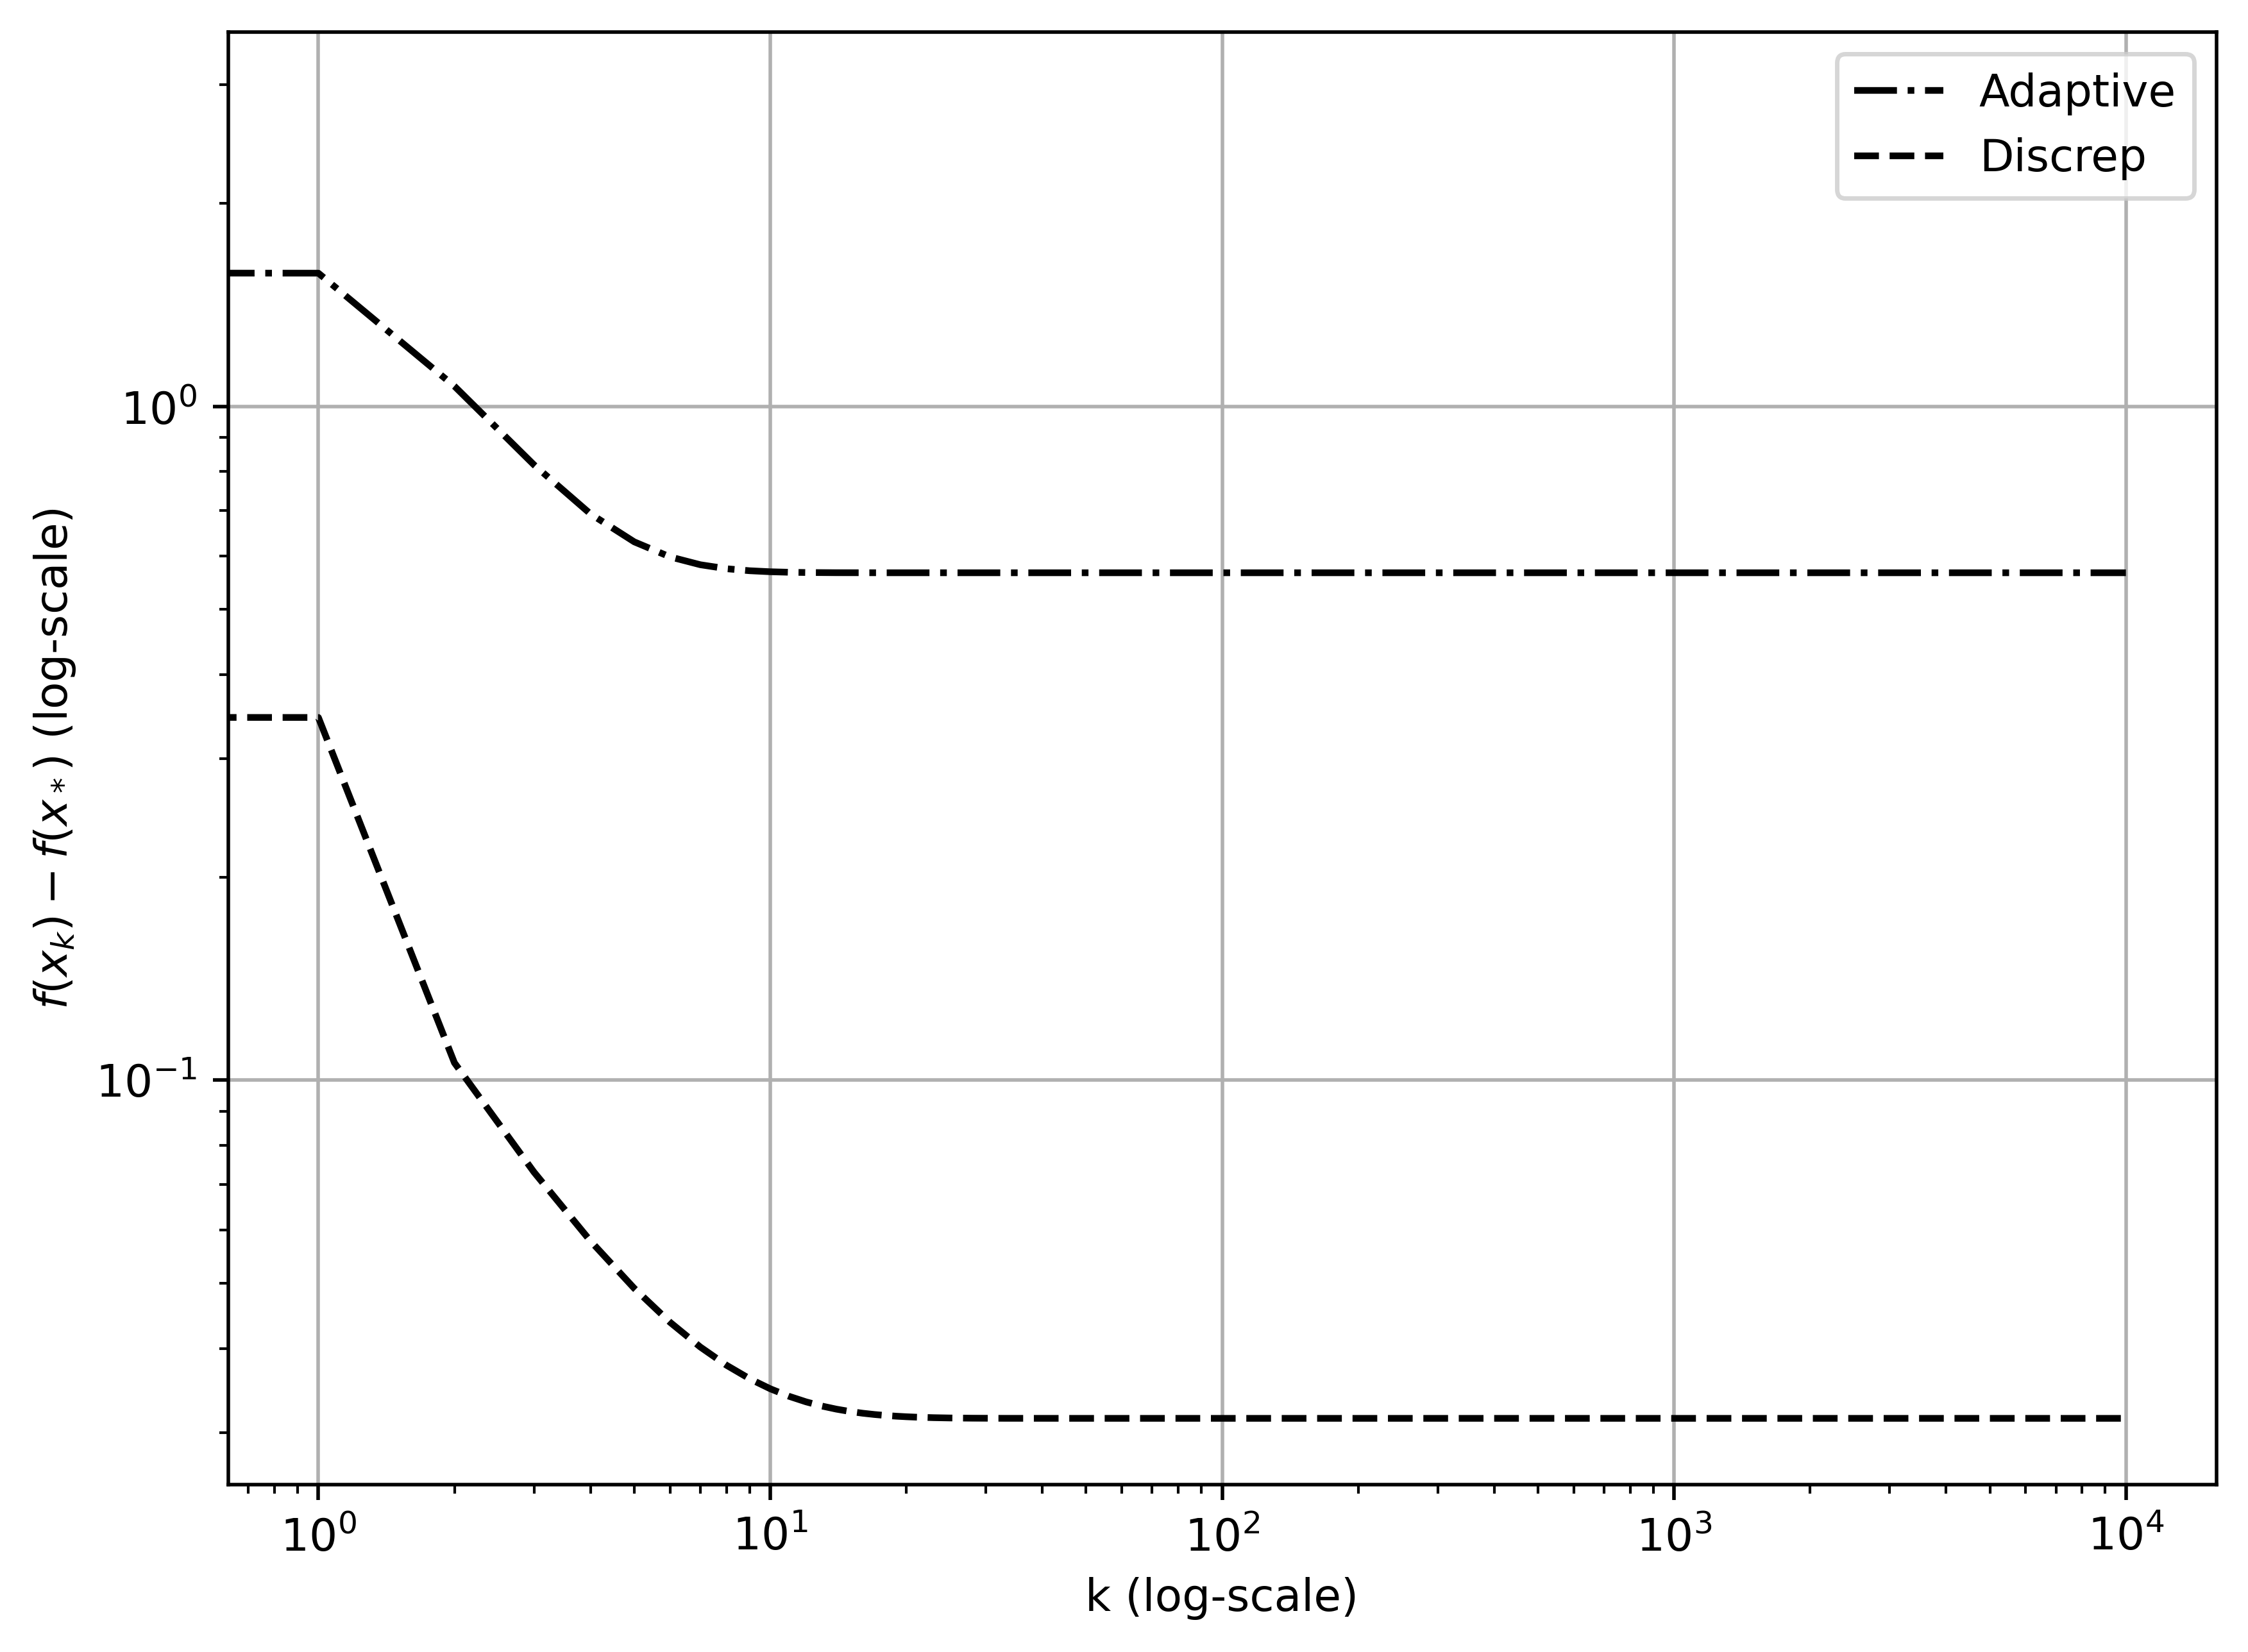
\includegraphics[width=\linewidth]{sharp_convex_f.png}
    \endminipage\hfill
    \caption{ Результаты решения задачи минимизации (\ref{allpha_sphere_cover}), где  $n= 1\,000, r = 0.7525, \alpha = 0.6$.}
    \label{res_sharp_convex}
\end{figure}

\begin{figure}[h]
    \minipage{0.49\textwidth}
    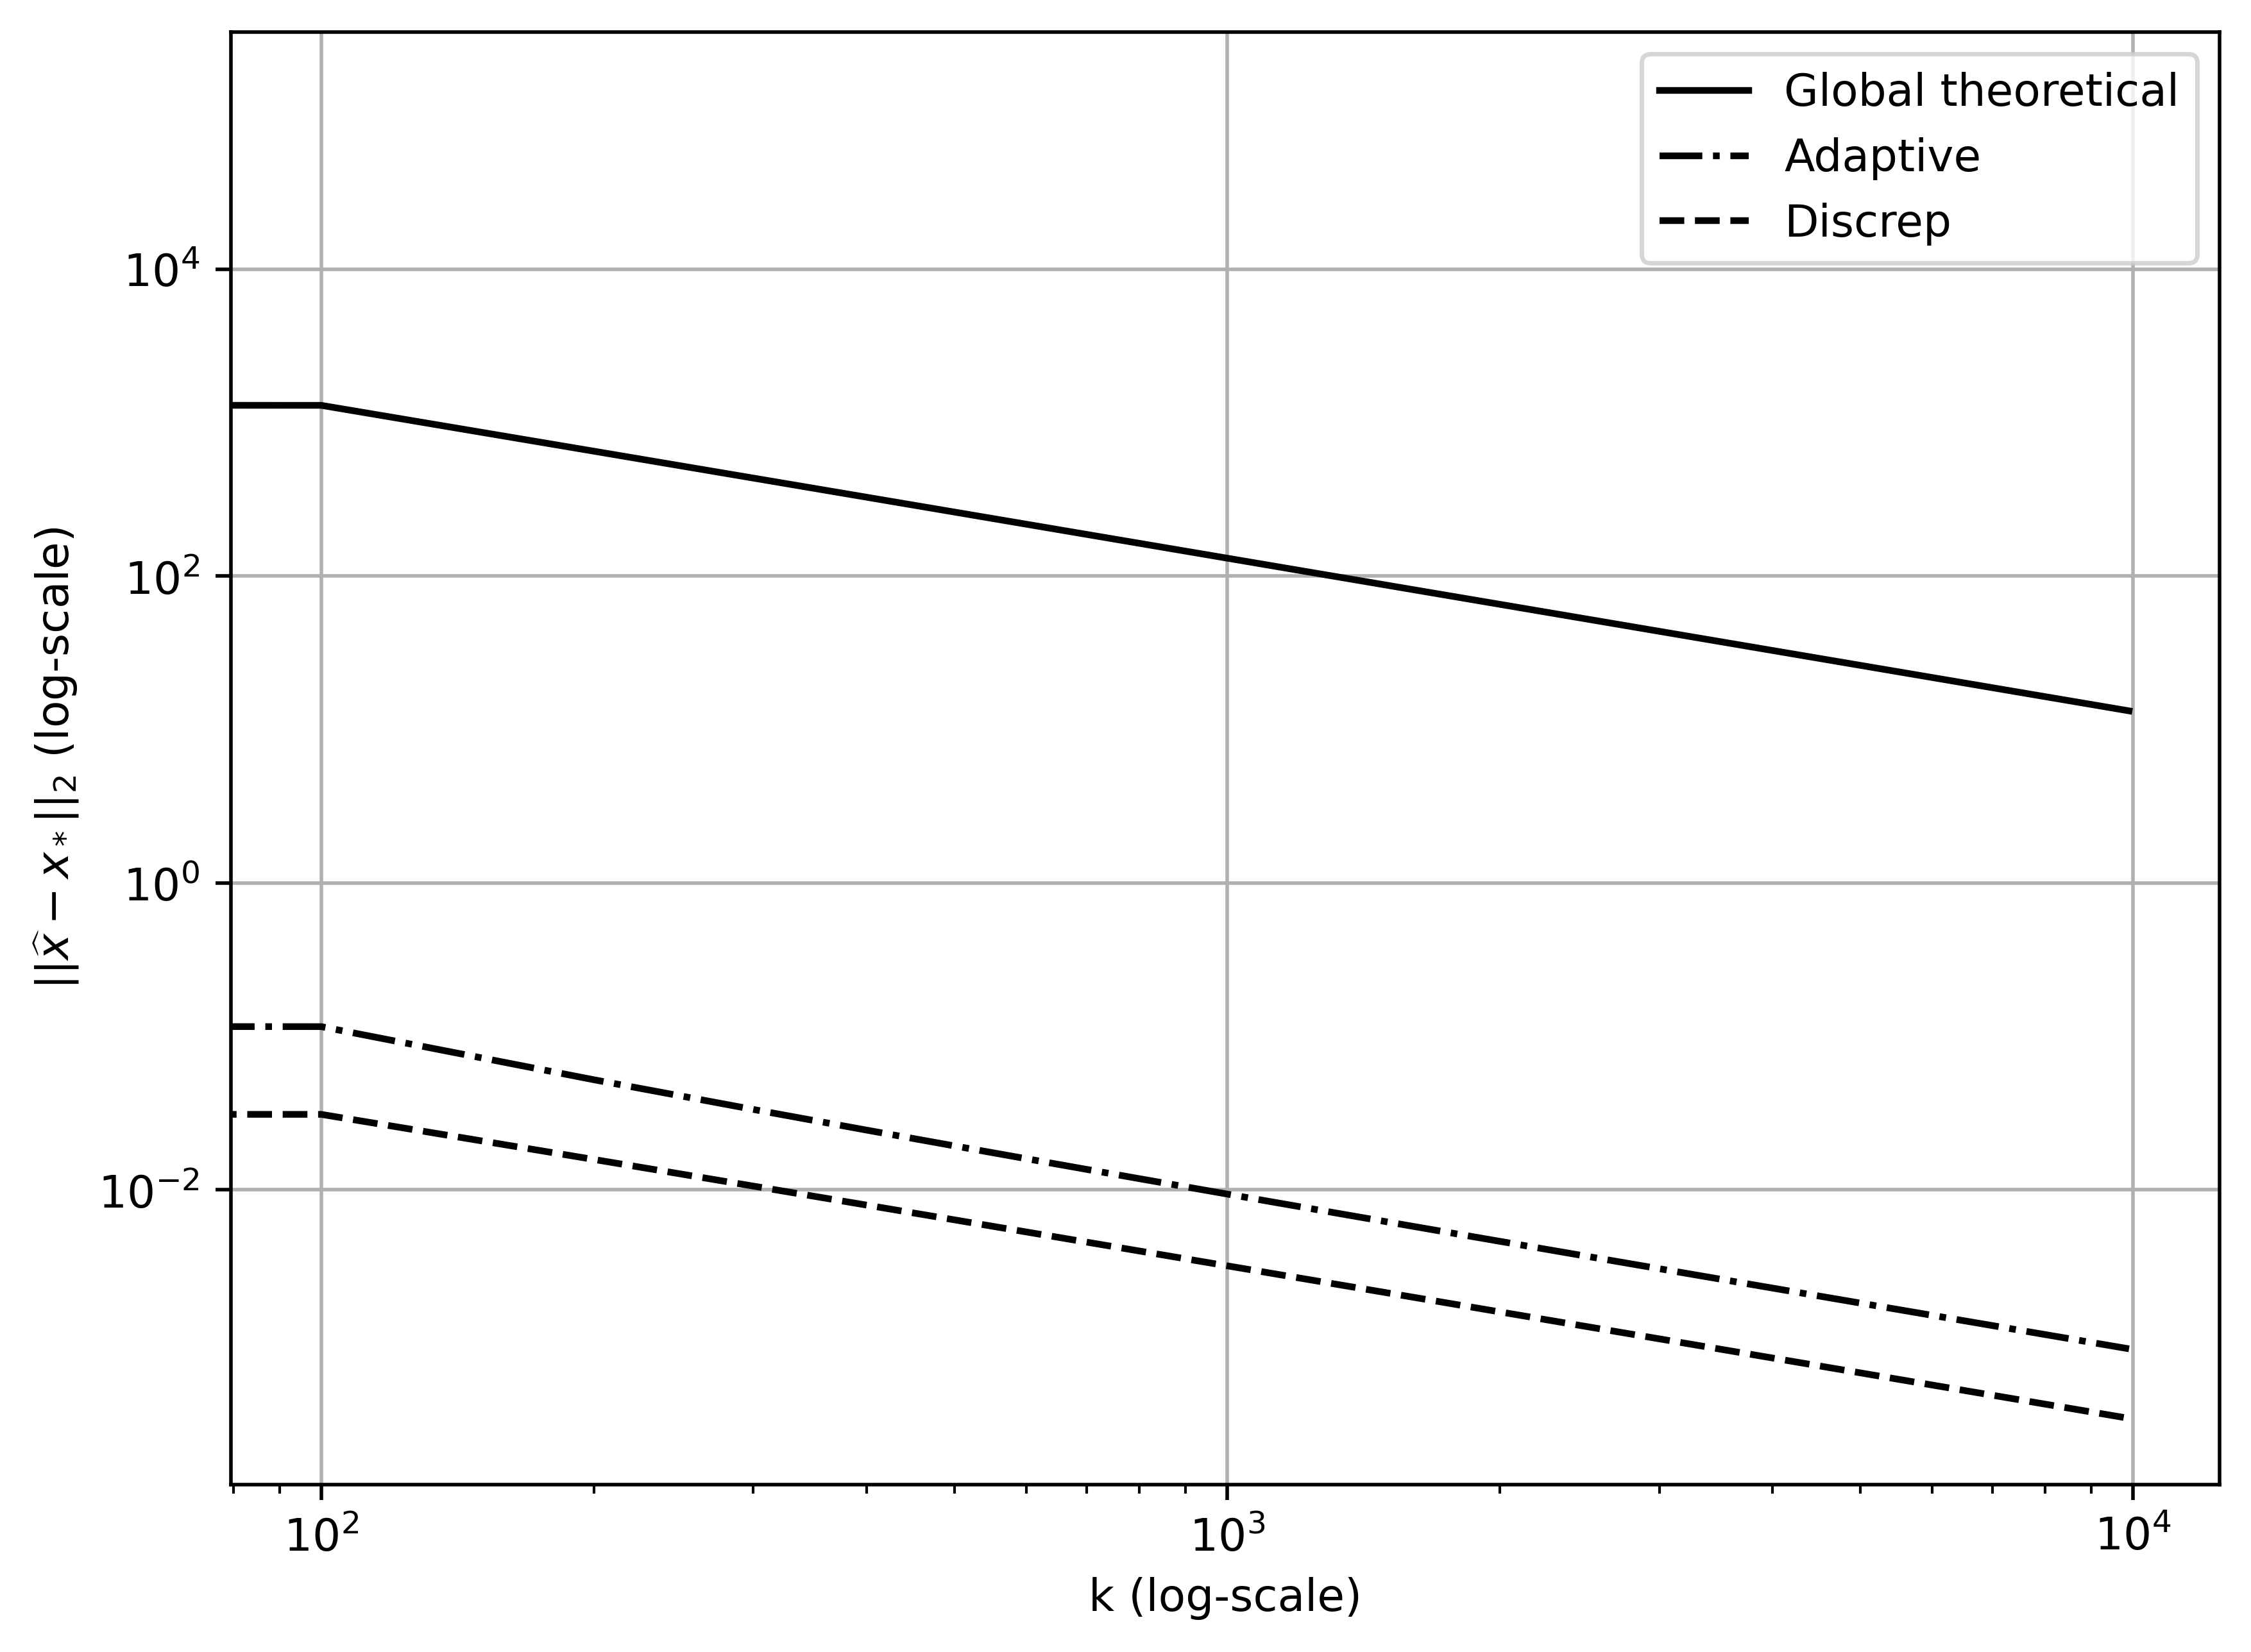
\includegraphics[width=\linewidth]{strong_convex_small_rad_x.png}
    \endminipage\hfill
    \minipage{0.49\textwidth}
    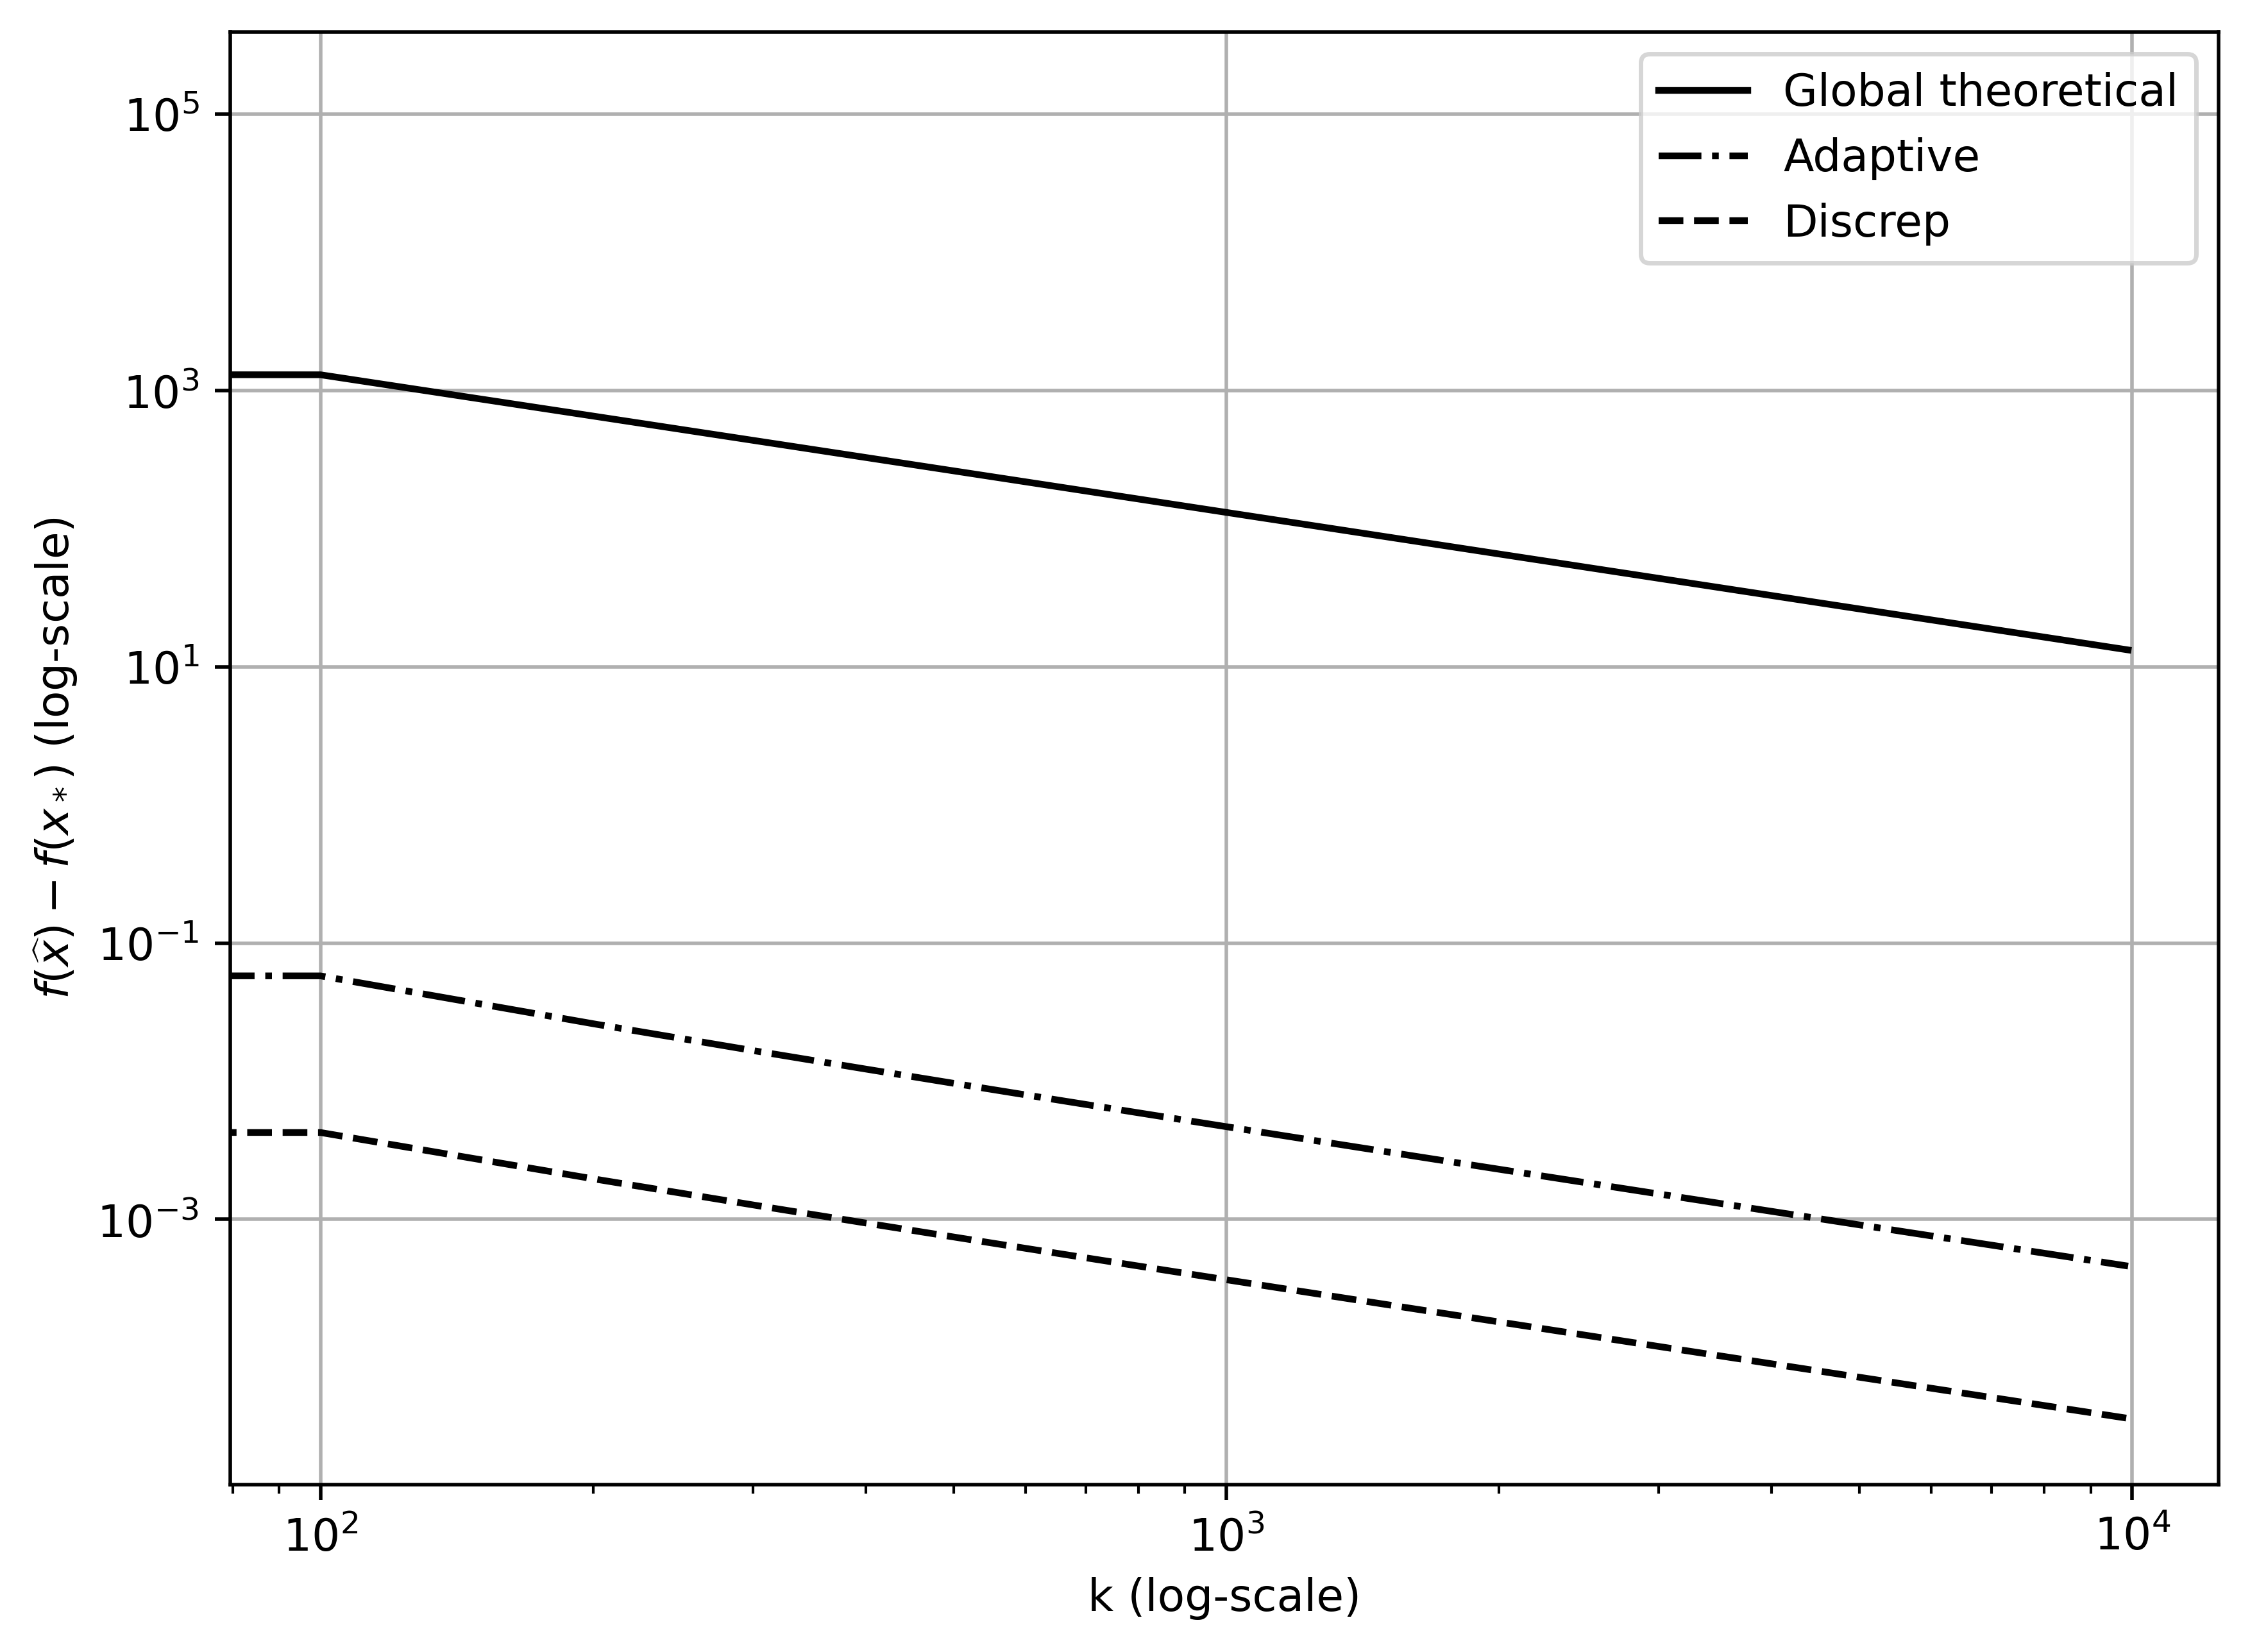
\includegraphics[width=\linewidth]{strong_convex_small_rad_f.png}
    \endminipage\hfill
    \caption{ Результаты решения задачи минимизации (\ref{sphere_cover_strongly}), где  $n= 1\,000, r = 0.7525$.}
    \label{res_strong_convex}
\end{figure}


\underline{\textbf{В параграфе 3.2}} вводится аналог условия острого минимума, а именно - условие относительного гамма роста. На его основе к методу классического зеркального спуска применяется схема рестартов, что позволяет улучшить получаемые оценки.
Воспользуемся следующим результатом из \cite{Lu_2018}:
\begin{theorem} \label{vanilla_mirror}
    Пусть $f$ --- является $M$-липшицевой на $Q$ относительно некоторой функции Брэгмана $V(x, y)$ c сильно выпуклой прокс-функцией $d(x)$. Тогда можно задать метод следующим образом:
    \begin{equation} \label{mirr_upd}
        x_{k+1} = \arg \min_{x \in Q} {\left[ f(x_k) + \langle \nabla f(x_k), x - x_k \rangle + \frac{1}{h_k} V(x, x_k)\right]},
    \end{equation}
    где $\{ h_k \}$ - последовательность размеров шагов.
    Для него справедлива следующая оценка скорости сходимости:
    \begin{equation} \label{general_est}
        \min_{0\leq k \leq N} f(x_k) - f(x) \leq \frac{\frac{1}{2} M^2 \sum_{k=0}^N h_k^2 + V(x, x_0)}{\sum_{k=0}^N h_k}
    \end{equation}
\end{theorem}

\begin{remark}
    Если в \eqref{mirr_upd} в формулировке теоремы \ref{vanilla_mirror} выбрать шаг следующим образом:
    \begin{equation} \label{mirr_step}
        h_{k} = \frac{\sqrt{2 \left[\min\limits_{x_* \in X_*}{V(x_*, x_0)}\right] }}{M\sqrt{N}},
    \end{equation}
    то можно выписать такую оценку скорости сходимости:
    \begin{equation} \label{mirr_est}
        f(\widehat{x_N}) - f(x_*) \leq \frac{M\sqrt{2 \left[\min\limits_{x_* \in X_*}{V(x_*, x_0)}\right]}}{\sqrt{N}}
    \end{equation}
\end{remark}
Если функция обладает дополнительными свойствами, аналогичными <<острому минимуму>>,  то становится возможным применение техники рестартов. Используем аналог данного условия и вслед за Шапиро–Немировским (см. \cite{shapiro_2005} и \cite{shapiro_2021} ) впервые введем условие относительного $\gamma$-роста ($\gamma \geq 1$). Отметим, что подобное условие впервые вводится с использованием дивергенции Брэгмана, что позволяет обобщить ряд условий, таких как условия <<острого минимума>>, <<квадратичного доминирования>> и <<$\gamma$-роста>>:
\begin{definition}
   $f$ --- удовлетворяет условию относительного $\gamma$-роста при условии:
   \begin{equation} \label{gamma-growth}
       f(x) - f(x_*) \geq \mu_{\gamma}\left(\min_{x_* \in X_*}{V(x_*,x)}\right)^{\gamma/2} \;\;\; \forall x \in Q,
   \end{equation}
   где $X_*$ --- множество возможный решений.  
\end{definition}

В данных предположениях была сформулирована и доказана следующая теорема:
\begin{theorem} \label{simple_restart}
    Пусть $f$ --- удовлетворяет условию относительного $\gamma$-роста \eqref{gamma-growth} и также является $M$-липшицевой на $Q$ относительно некоторой функции Брэгмана $V(x, y)$. В таком случае Алгоритм \ref{alg:rest_gamma} достигнет точности $\epsilon$ за:
    \begin{equation}
    \begin{aligned}
       N =\mathcal{O}\left(\frac{2 M^2}{\mu_{\gamma}^2} \log_2{\frac{\min\limits_{x_* \in X_*}{V(x_*, x_0^0)}}{\varepsilon}}\right) \text{ при } \gamma = 1, \\
       N = \mathcal{O}\left(\frac{2^{\gamma + 1} M^2}{\mu_{\gamma}^2 (2^{\gamma} - 2)} \left[\varepsilon^{(1 - \gamma)} - \left(\min\limits_{x_* \in X_*}{V(x_*, x_0^0)}\right)^{(1 - \gamma)}\right]\right) \text{ при } \gamma > 1,
    \end{aligned}
    \end{equation}
    обращений к субградиенту, причем будут справедливы неравенства:
    \begin{equation}
        \min_{x_* \in X_*}{V(x_*, \widehat{x_p})} \leq \varepsilon
    \end{equation}
    и
    \begin{equation}
        f(\widehat{x_p}) - f(x_*) \leq M \sqrt{2 \varepsilon}.  
    \end{equation}
\end{theorem}

\begin{algorithm}[htp]
    \caption{Рестарты зеркального спуска при условии относительного $\gamma$-роста.}
    \label{alg:rest_gamma}
    \KwData{$\varepsilon > 0$}
    \KwResult{$x_p$}
    $p \gets 0$\;
    $\min\limits_{x_* \in X_*}{V(x_*, x_0)} \gets \min\limits_{x_* \in X_*}{V(x_*,x_0^0)}$\;
    \While{$p < \log_2\left(\frac{\min\limits_{x_* \in X_*}{V(x_*, x_0^0)}}{\varepsilon}\right).$}{
        $x_{p}$ --- результат работы метода \eqref{mirr_upd} с шагом \eqref{mirr_step} и параметром $N_{p} = \ceil*{\frac{M^2 2^{\gamma}}{\mu_{\gamma}^2 2^{p(1 - \gamma)}} \left(\min\limits_{x_* \in X_*}{V(x_*, x_0^0)}\right)^{1 - \gamma}}$\;
        $x_0 = \widehat{x_p}$\;
        $\min\limits_{x_* \in X_*}{V(x_*, x_0)} \gets \frac{1}{2^{p+1}}\min\limits_{x_* \in X_*}{V_{0}(x_*, x_0^0)}$\;
        $p=p+1$\;
    }
\end{algorithm}

Также путем замены $\delta := M \sqrt{2 \varepsilon}$ в предыдущей теореме, можно сформулировать следующее замечание:
\begin{remark}
    Пусть $f$ --- удовлетворяет условию $\gamma$-роста \eqref{gamma-growth} и также является $M$-липшицевой на $Q$ относительно некоторой дивергенции Брэгмана $V(x, y)$. В таком случае, Алгоритм \ref{alg:rest_gamma} достигнет точности $\delta$ за:
    \begin{equation}
        \begin{aligned}
           N = \mathcal{O}\left(\frac{2 M^2}{\mu_{\gamma}^2} \log_2{\frac{2 M^2 \left[\min\limits_{x_* \in X_*}{V(x_*, x_0^0)}\right]}{\delta^2}}\right) \text{ при } \gamma = 1, \\
           N = \mathcal{O}\left(\frac{2^{\gamma + 1} M^2}{\mu_{\gamma}^2 (2^{\gamma} - 2)} \left[\left(\frac{\delta^2}{2 M^2}\right)^{(1 - \gamma)} - \left(\min\limits_{x_* \in X_*}{V(x_*, x_0^0)}\right)^{(1 - \gamma)}\right]\right) \text{ при } \gamma > 1,
        \end{aligned}
    \end{equation}
    обращений к субградиенту $f$, причем будут справедливы неравенства:
    \begin{equation}
       f(\widehat{x_p}) - f(x_*)  \leq \delta 
    \end{equation}
    и
    \begin{equation}
       \min\limits_{x_* \in X_*}{V(x_*, \widehat{x_p})} \leq \frac{\delta^2}{2 M^2}.
    \end{equation}
\end{remark}

\underline{\textbf{В параграфе 3.3}} предлагается развитие полученных в предыдущем параграфе результатов. На практике для использования приведенной выше теоремы \ref{simple_restart} требуется знание о точном решении для оценки $\min\limits_{x_* \in X_*}{V(x_*, x_0^0)}$, что лишает данный метод практической пользы. Потому стоит провести замену расстояния Брэгмана оценкой сверху:
\begin{equation} \label{adapt_est_theta}
\begin{aligned}
    \min_{0\leq k \leq N} f(x_k) - f(x_*) \leq \frac{\sum_{k=0}^N h_k^2 \norm{\nabla f(x_k)}^2} {2 \sum_{k=0}^N h_k} + \frac{\min\limits_{x_* \in X_*}{V(x_*, x_0)} }{\sum_{k=0}^N h_k} \leq \\
    \leq \frac{\sum_{k=0}^N h_k^2 \norm{g(x_k)}^2} {2 \sum_{k=0}^N h_k} + \frac{\Theta^2}{\sum_{k=0}^N h_k}.
\end{aligned}
\end{equation}
Также для дальнейших рассуждений потребуется более точная оценка, чем \eqref{general_est}. Доказывается справедливость следующего результата:
\begin{remark} \label{adapt_mirror}
    Пусть $f$ --- является $M$-липшицевой на $Q$ относительно некоторой функции Брэгмана $V(x, y)$ c 1-сильно выпуклой прокс-функцией $d(x)$.
    Зададим метод аналогично теореме \ref{vanilla_mirror}: 
    \begin{equation} \label{adapt_upd}
        x_{k+1} = \arg \min_{x \in Q} {\left[ f(x_k) + \langle \nabla f(x_k), x - x_k \rangle + \frac{1}{h_k} V(x, x_k)\right]},
    \end{equation}
    где $\{ h_k \}$ - последовательность размеров шагов. Тогда справедлива следующая оценка:
    \begin{equation} \label{adapt_est}
        \min_{0\leq k \leq N} f(x_k) - f(x_*) \leq \frac{\sum_{k=0}^N h_k^2 \norm{\nabla f(x_k)}^2} {2 \sum_{k=0}^N h_k} + \frac{\min\limits_{x_* \in X_*}{V(x_*, x_0)} }{\sum_{k=0}^N h_k}.
    \end{equation}
\end{remark}

Данный вспомогательный результат позволяет провести замену глобальной константы $M$ на локальные значения в теореме \ref{vanilla_mirror}. Что позволяет сформулировать критерий остановки метода для каждого из рестартов.
\begin{remark}
    Если в \eqref{adapt_upd} выбрать шаг следующим образом:
    \begin{equation} \label{eps_step}
        h_{k} = \frac{\varepsilon}{\norm{\nabla f(x_k)}^2},
    \end{equation}
    и воспользоваться критерием остановки метода на рестарте: 
    \begin{equation} \label{stop_crit}
        \sum_{k=0}^N \frac{1} {\norm{\nabla f(x_k)}^2} \geq \frac{2 \Theta^2}{\varepsilon^2}, \;\;\;\;\text{ где } \Theta \geq \min\limits_{x_* \in X_*}{V(x_*, x_0)},
    \end{equation}
    тогда для невязки по функции будет справедливо следующее:
    \begin{equation} 
    \begin{aligned}
        \min_{0\leq k \leq N} f(x_k) - f(x_*) \leq \frac{\varepsilon}{2} + \frac{\Theta^2}{\varepsilon \sum_{k=0}^N \frac{1} {\norm{\nabla f(x_k)}^2}} \leq \varepsilon.
    \end{aligned}
    \end{equation}
 \end{remark}

 Все вспомогательные результаты, полученные ранее, дают возможность объединить их и сформулировать в виде удобного с практической точки зрения алгоритма. Данный алгоритм требует оценки сверху для расстояния от начальной точки до точного решения, которая может быть сколь угодно <<грубой>>. Это позволяет в дальнейшем усложнять алгоритм, подбирая лучшую начальную оценку расстояния. Также соответствующая теорема \ref{restared_criteria} показывает, что даже существенно <<ослабленная>> версия условия <<острого>> минимума позволяет значимо повысить скорость сходимости.

\begin{algorithm}[htp]
    \caption{Рестарты зеркального спуска при условии $\gamma$-роста с критерием остановки.}
    \label{alg:rest_criteria}
    \KwData{$\varepsilon > 0$}
    \KwResult{$x_p$}
    $p \gets 0$\;
    $\Theta_0 \geq \min\limits_{x_* \in X_*}{V(x_*,x_0^0)}$\;
    \While{$p < \log_2{\left[\left(\frac{\mu_{\gamma}}{\varepsilon}\right)^{\frac{2}{\gamma}} \frac{\Theta_0^2}{2}\right]}.$}{
        $x_{p}$ --- результат работы метода \eqref{mirr_upd} с шагом \eqref{eps_step} и критерием остановки $\sum_{k=0}^{N_p} \frac{1}{\norm{\nabla f(x_k) }_2^2} \geq \frac{ 2^{(p \gamma - p + \gamma + 1)}}{\mu_{\gamma}^2 \Theta_0^{2\gamma - 2} } $\;
        $x_0 = x_{min}^p$\;
        $p=p+1$\;
    }
\end{algorithm}
\begin{theorem} \label{restared_criteria}
    Пусть $f$ --- удовлетворяет условию $\gamma$-роста \eqref{gamma-growth} и также является $M$-липшицевой на $Q$ относительно некоторой функции Брэгмана $V(x, y)$. В таком случае Алгоритм \ref{alg:rest_criteria} достигнет точности $\varepsilon$ за:
    \begin{equation}
       N = \mathcal{O} \left( \frac{4 M^2}{\mu_{\gamma}^2} \log_2{\left[\left(\frac{\mu_{\gamma}}{\varepsilon}\right)^{\frac{2}{\gamma}} \frac{\Theta_0^2}{2}\right]}\right) \text{ при } \gamma = 1
   \end{equation}
   или
   \begin{equation}
       N = \mathcal{O}\left( \frac{2 M^2 }{2^{\gamma - 1} - 1}\left[ \frac{2}{\mu_{\gamma}^{\frac{2}{\gamma}}}\varepsilon^{\frac{2}{\gamma} - 2} - \frac{2^{\gamma}}{\mu_{\gamma}^2 \Theta_0^{2(\gamma - 1)}} \right] \right) \text{ при } \gamma > 1.
   \end{equation}
\end{theorem}

 Полученный результат имеет схожие оценки с предыдущей теоремой \ref{simple_restart}, однако на практике критерий остановки значительно сокращает количество итераций, необходимых для достижения заданной точности $\varepsilon$. Также при помощи данного метода легко прогнозируется точность перед каждым рестартом метода, что удобно для контроля за правильностью работы метода. Также подобная информация позволяет переключаться между несколькими модификациями метода, чередуя не только "эффективные" и "аналитические" шаги, но и перезапуски.  

\FloatBarrier
\pdfbookmark{Заключение}{conclusion}                                  % Закладка pdf
В \underline{\textbf{заключении}} приведены основные результаты работы, которые заключаются в следующем:
%% Согласно ГОСТ Р 7.0.11-2011:
%% 5.3.3 В заключении диссертации излагают итоги выполненного исследования, рекомендации, перспективы дальнейшей разработки темы.
%% 9.2.3 В заключении автореферата диссертации излагают итоги данного исследования, рекомендации и перспективы дальнейшей разработки темы.
\begin{enumerate}
  \item Доказаны оптимальные оценки для зеркального спуска для вариационных неравенств с относительно сильно монотонными и относительно ограниченными операторами с точностью до умножения на постоянный множитель.
  \item Получена адаптивная оценка скорости сходимости зеркального спуска для задач минимизации сильно выпуклых функций с использованием локальных аналогов константы Липшица.  
  \item Доказана оценка скорости сходимости рестартованного метода зеркального спуска для относительно липшицевых задач оптимизации с относительным  $\gamma$-ростом.
  \item Предложены адаптивные правила остановки для рестартов исследуемого метода зеркального спуска в предположении липшицевости и 
  $\gamma$-ростом целевой функции и получены теоретические оценки сложности такой  процедуры. 
  \item Проведено исследование и сравнение практической работы методов безградиентного, градиентного и квазинютоновского типов для минимизации функционала OPLS force field, отвечающего за минимизацию энергии белка.
  \item Реализована вспомогательная библиотека для экспериментальной проверки исследуемых в работе субградиентных методов. 
\end{enumerate}


\pdfbookmark{Литература}{bibliography}                                % Закладка pdf


\ifdefmacro{\microtypesetup}{\microtypesetup{protrusion=false}}{} % не рекомендуется применять пакет микротипографики к автоматически генерируемому списку литературы
\urlstyle{rm}                               % ссылки URL обычным шрифтом
\ifnumequal{\value{bibliosel}}{0}{% Встроенная реализация с загрузкой файла через движок bibtex8
    \renewcommand{\bibname}{\large \bibtitleauthor}
    \nocite{*}
    \insertbiblioauthor           % Подключаем Bib-базы
    %\insertbiblioexternal   % !!! bibtex не умеет работать с несколькими библиографиями !!!
}{% Реализация пакетом biblatex через движок biber
    % Цитирования.
    %  * Порядок перечисления определяет порядок в библиографии (только внутри подраздела, если `\insertbiblioauthorgrouped`).
    %  * Если не соблюдать порядок "как для \printbibliography", нумерация в `\insertbiblioauthor` будет кривой.
    %  * Если цитировать каждый источник отдельной командой --- найти некоторые ошибки будет проще.
    \nocite{Stonyakin_2021}%
    \nocite{yakovlev2019algorithms}%
    \nocite{sharp22}%
    \nocite{GorbunovKMR20}%
    %

    \ifnumgreater{\value{usefootcite}}{0}{
        \begin{refcontext}[labelprefix={}]
            \ifnum \value{bibgrouped}>0
                \insertbiblioauthorgrouped    % Вывод всех работ автора, сгруппированных по источникам
            \else
                \insertbiblioauthor      % Вывод всех работ автора
            \fi
        \end{refcontext}
    }{
        \ifnum \totvalue{citeexternal}>0
            \begin{refcontext}[labelprefix=A]
                \ifnum \value{bibgrouped}>0
                    \insertbiblioauthorgrouped    % Вывод всех работ автора, сгруппированных по источникам
                \else
                    \insertbiblioauthor      % Вывод всех работ автора
                \fi
            \end{refcontext}
        \else
            \ifnum \value{bibgrouped}>0
                \insertbiblioauthorgrouped    % Вывод всех работ автора, сгруппированных по источникам
            \else
                \insertbiblioauthor      % Вывод всех работ автора
            \fi
        \fi
        %  \insertbiblioauthorimportant  % Вывод наиболее значимых работ автора (определяется в файле characteristic во второй section)
        \begin{refcontext}[labelprefix={}]
            \insertbiblioexternal            % Вывод списка литературы, на которую ссылались в тексте автореферата
        \end{refcontext}
        % Невидимый библиографический список для подсчёта количества внешних публикаций
        % Используется, чтобы убрать приставку "А" у работ автора, если в автореферате нет
        % цитирований внешних источников.
        \printbibliography[heading=nobibheading, section=0, env=countexternal, keyword=biblioexternal, resetnumbers=true]%
    }
}
\ifdefmacro{\microtypesetup}{\microtypesetup{protrusion=true}}{}
\urlstyle{tt}                               % возвращаем установки шрифта ссылок URL
